%% LyX 2.3.6.1 created this file.  For more info, see http://www.lyx.org/.
%% Do not edit unless you really know what you are doing.
\documentclass[english]{article}
\usepackage[T1]{fontenc}
\usepackage[latin9]{inputenc}
\usepackage{graphicx}
\usepackage{babel}
\begin{document}
1.3

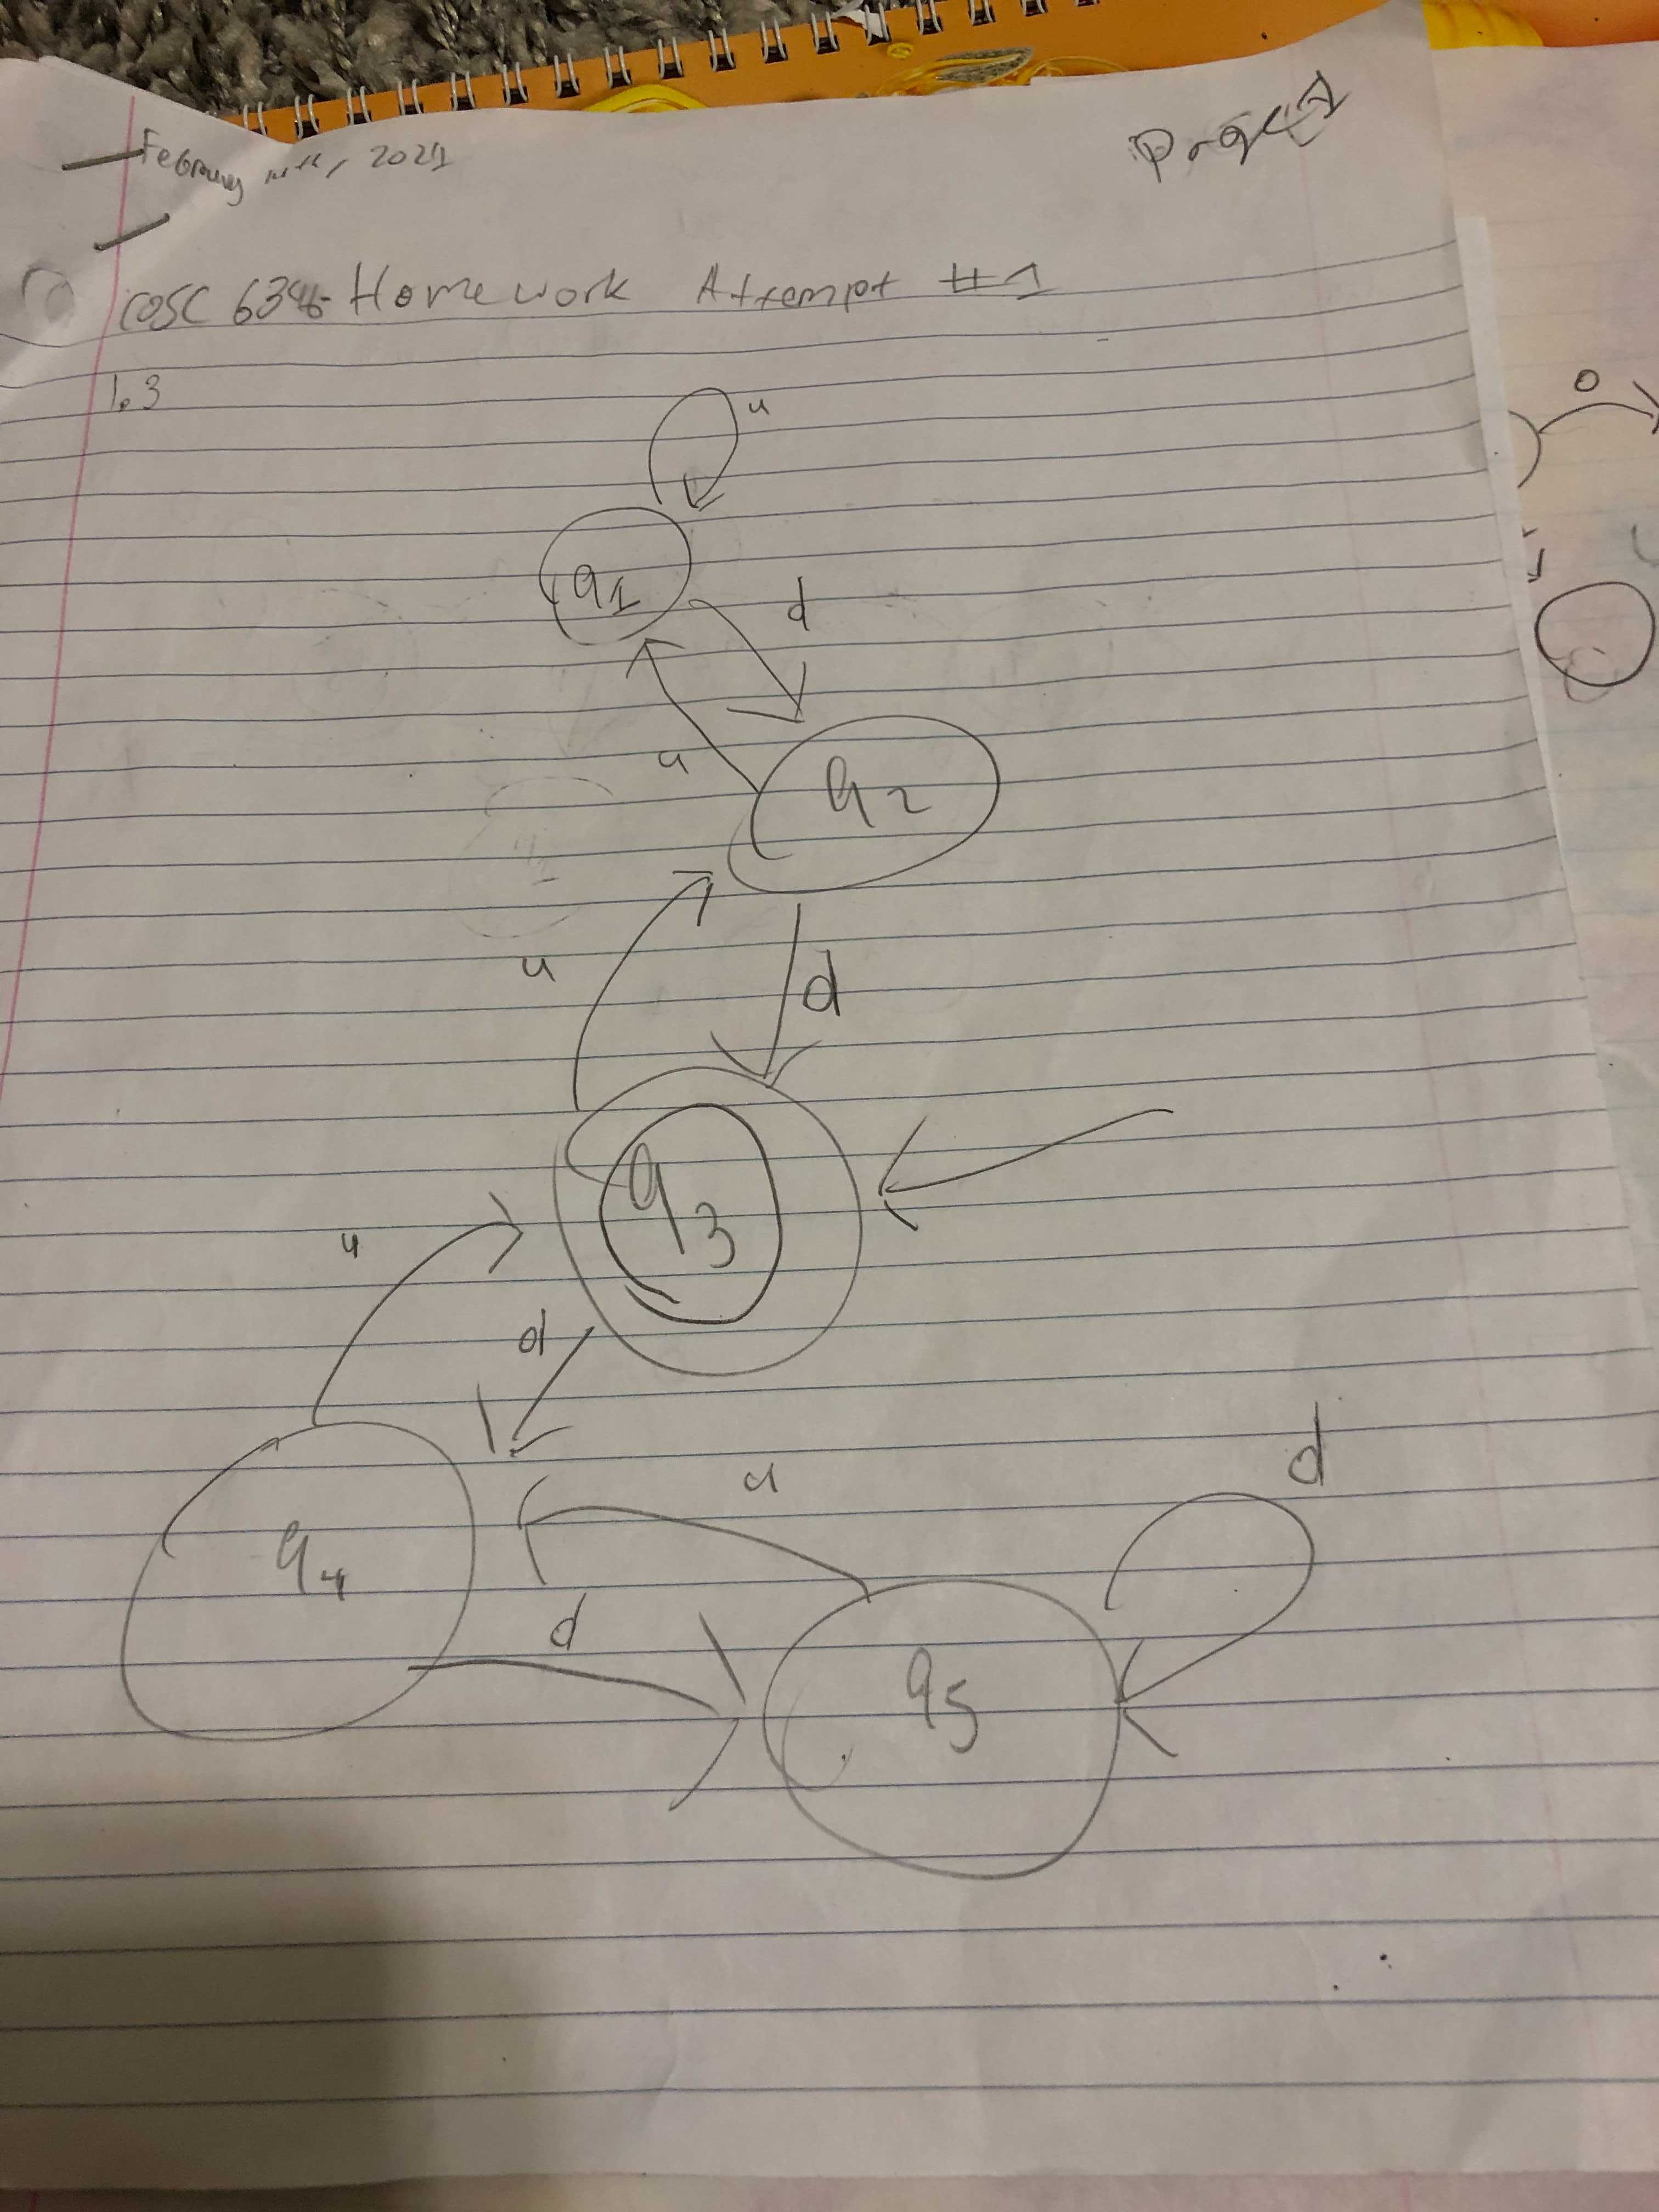
\includegraphics[width=15cm,height=15cm]{pics/page1}

1.6 

a.

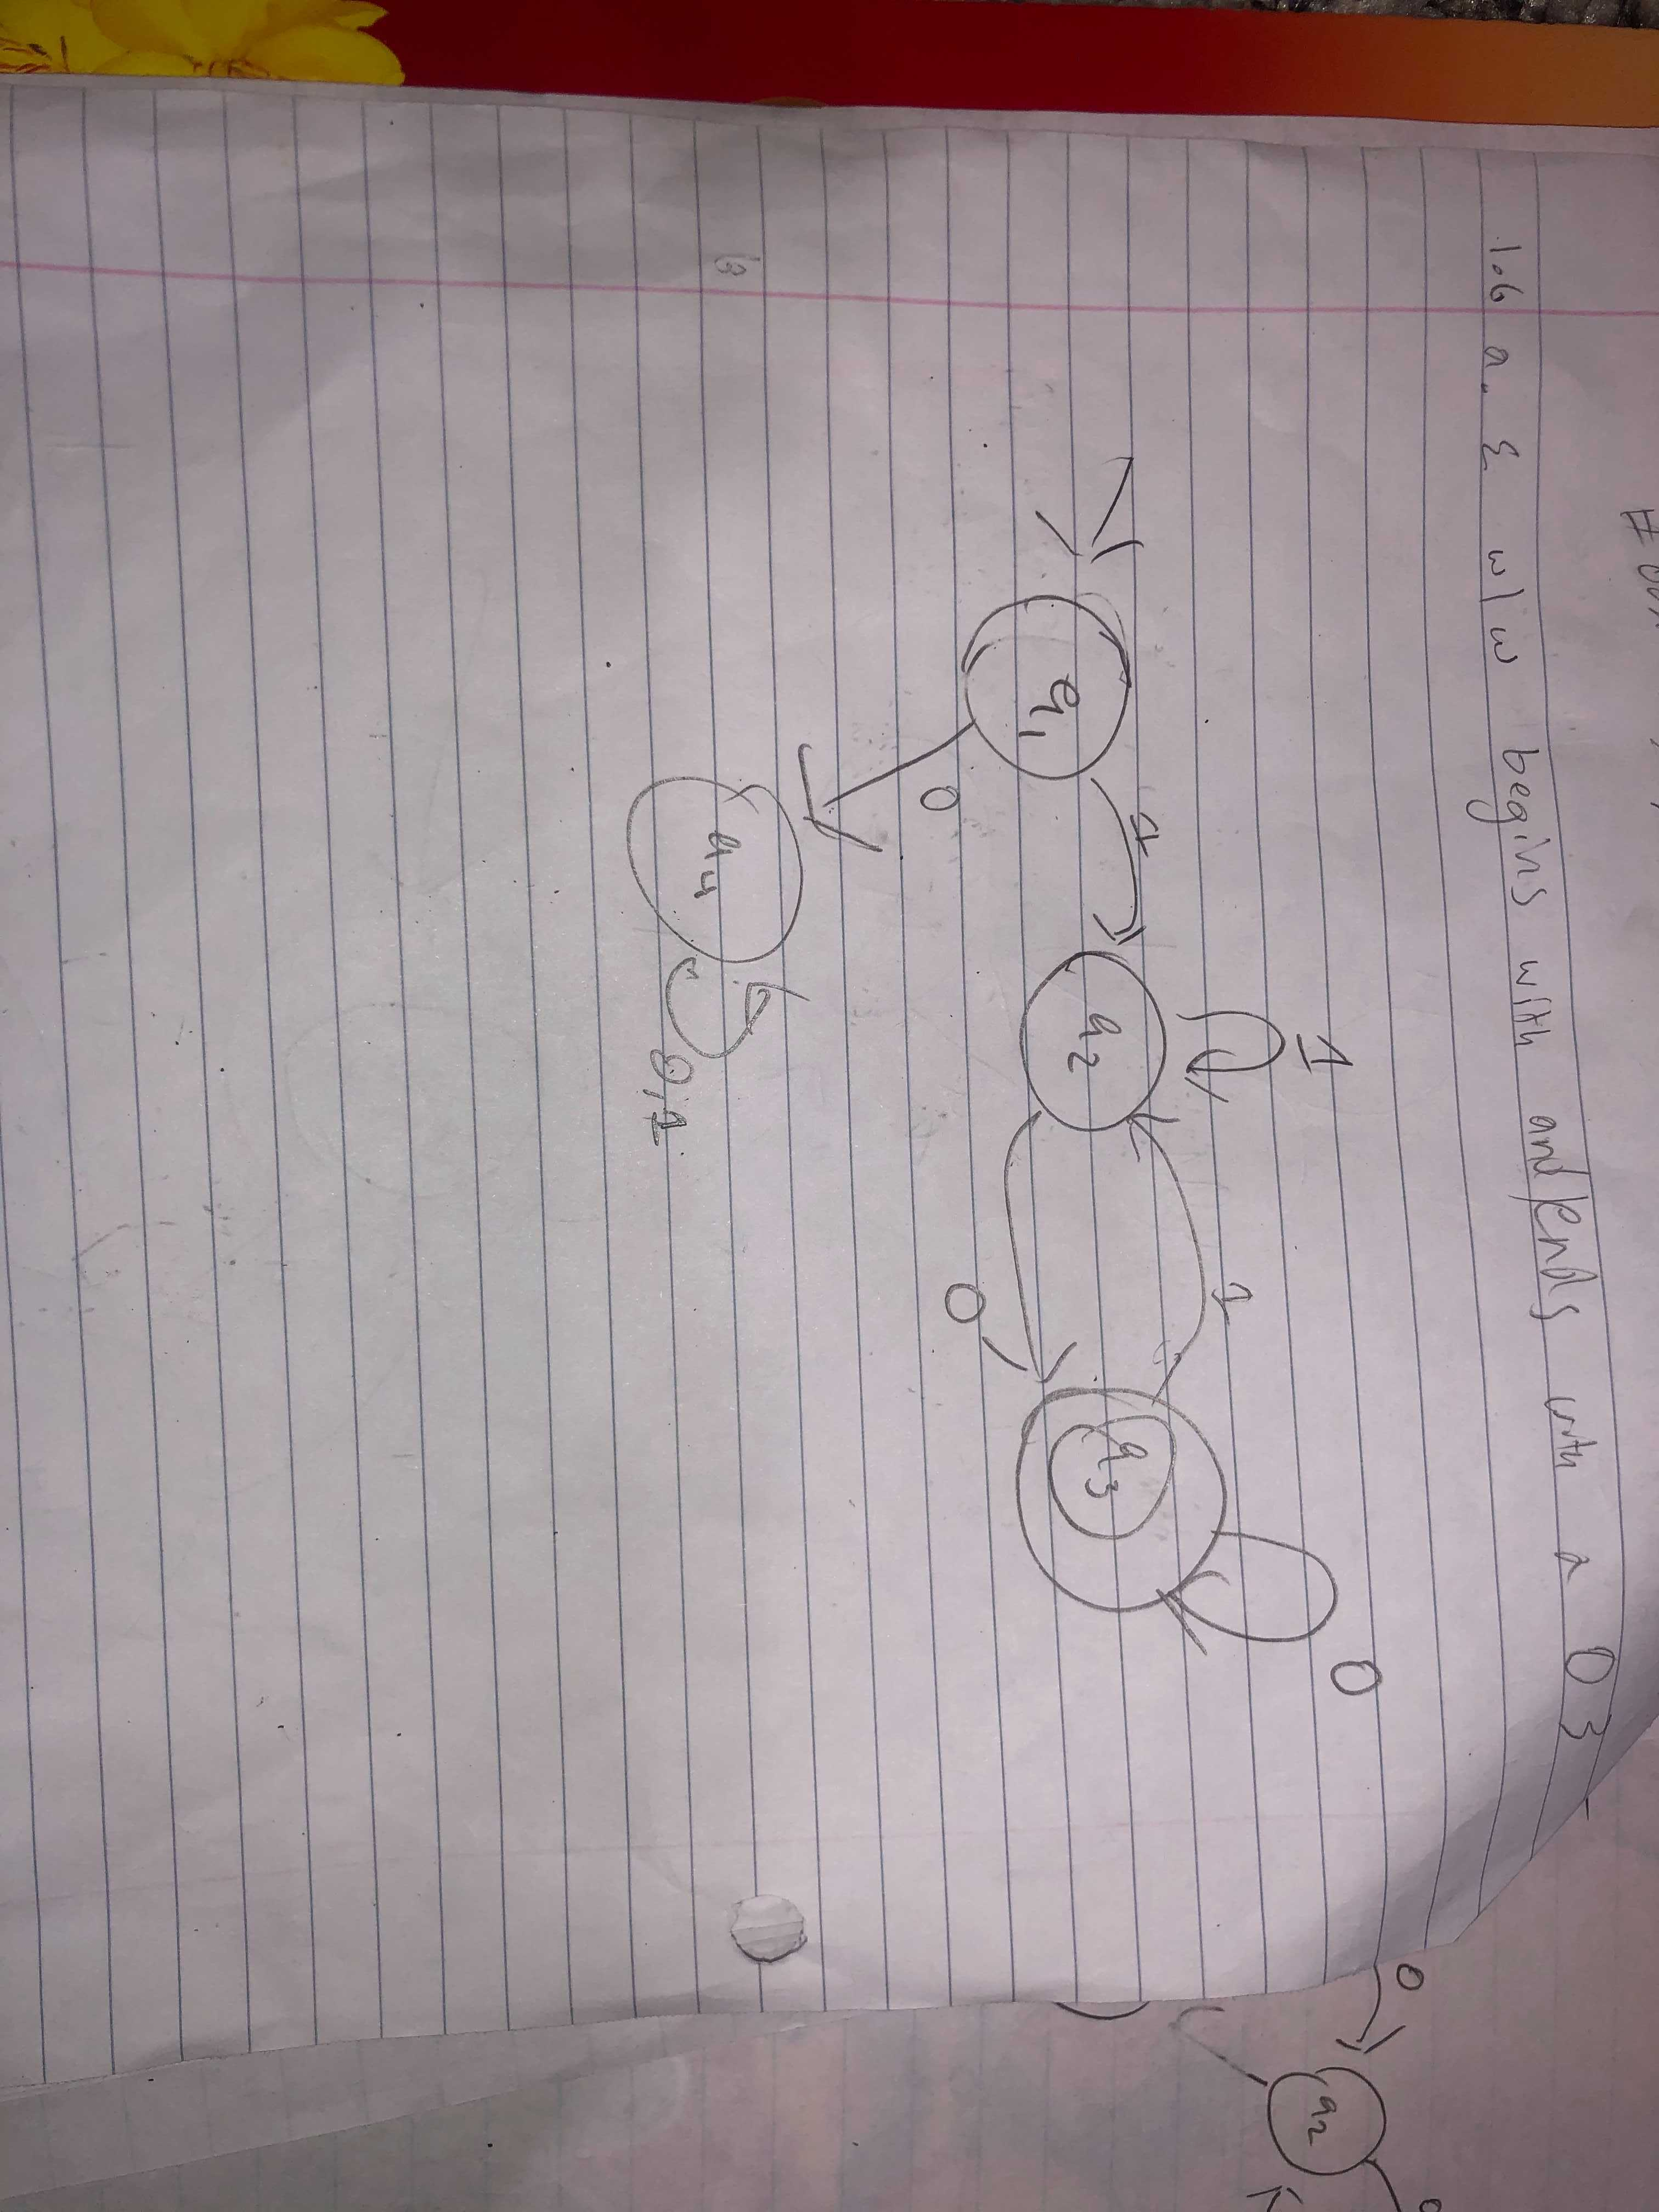
\includegraphics[width=15cm,height=15cm,keepaspectratio]{pics/page2}

b.

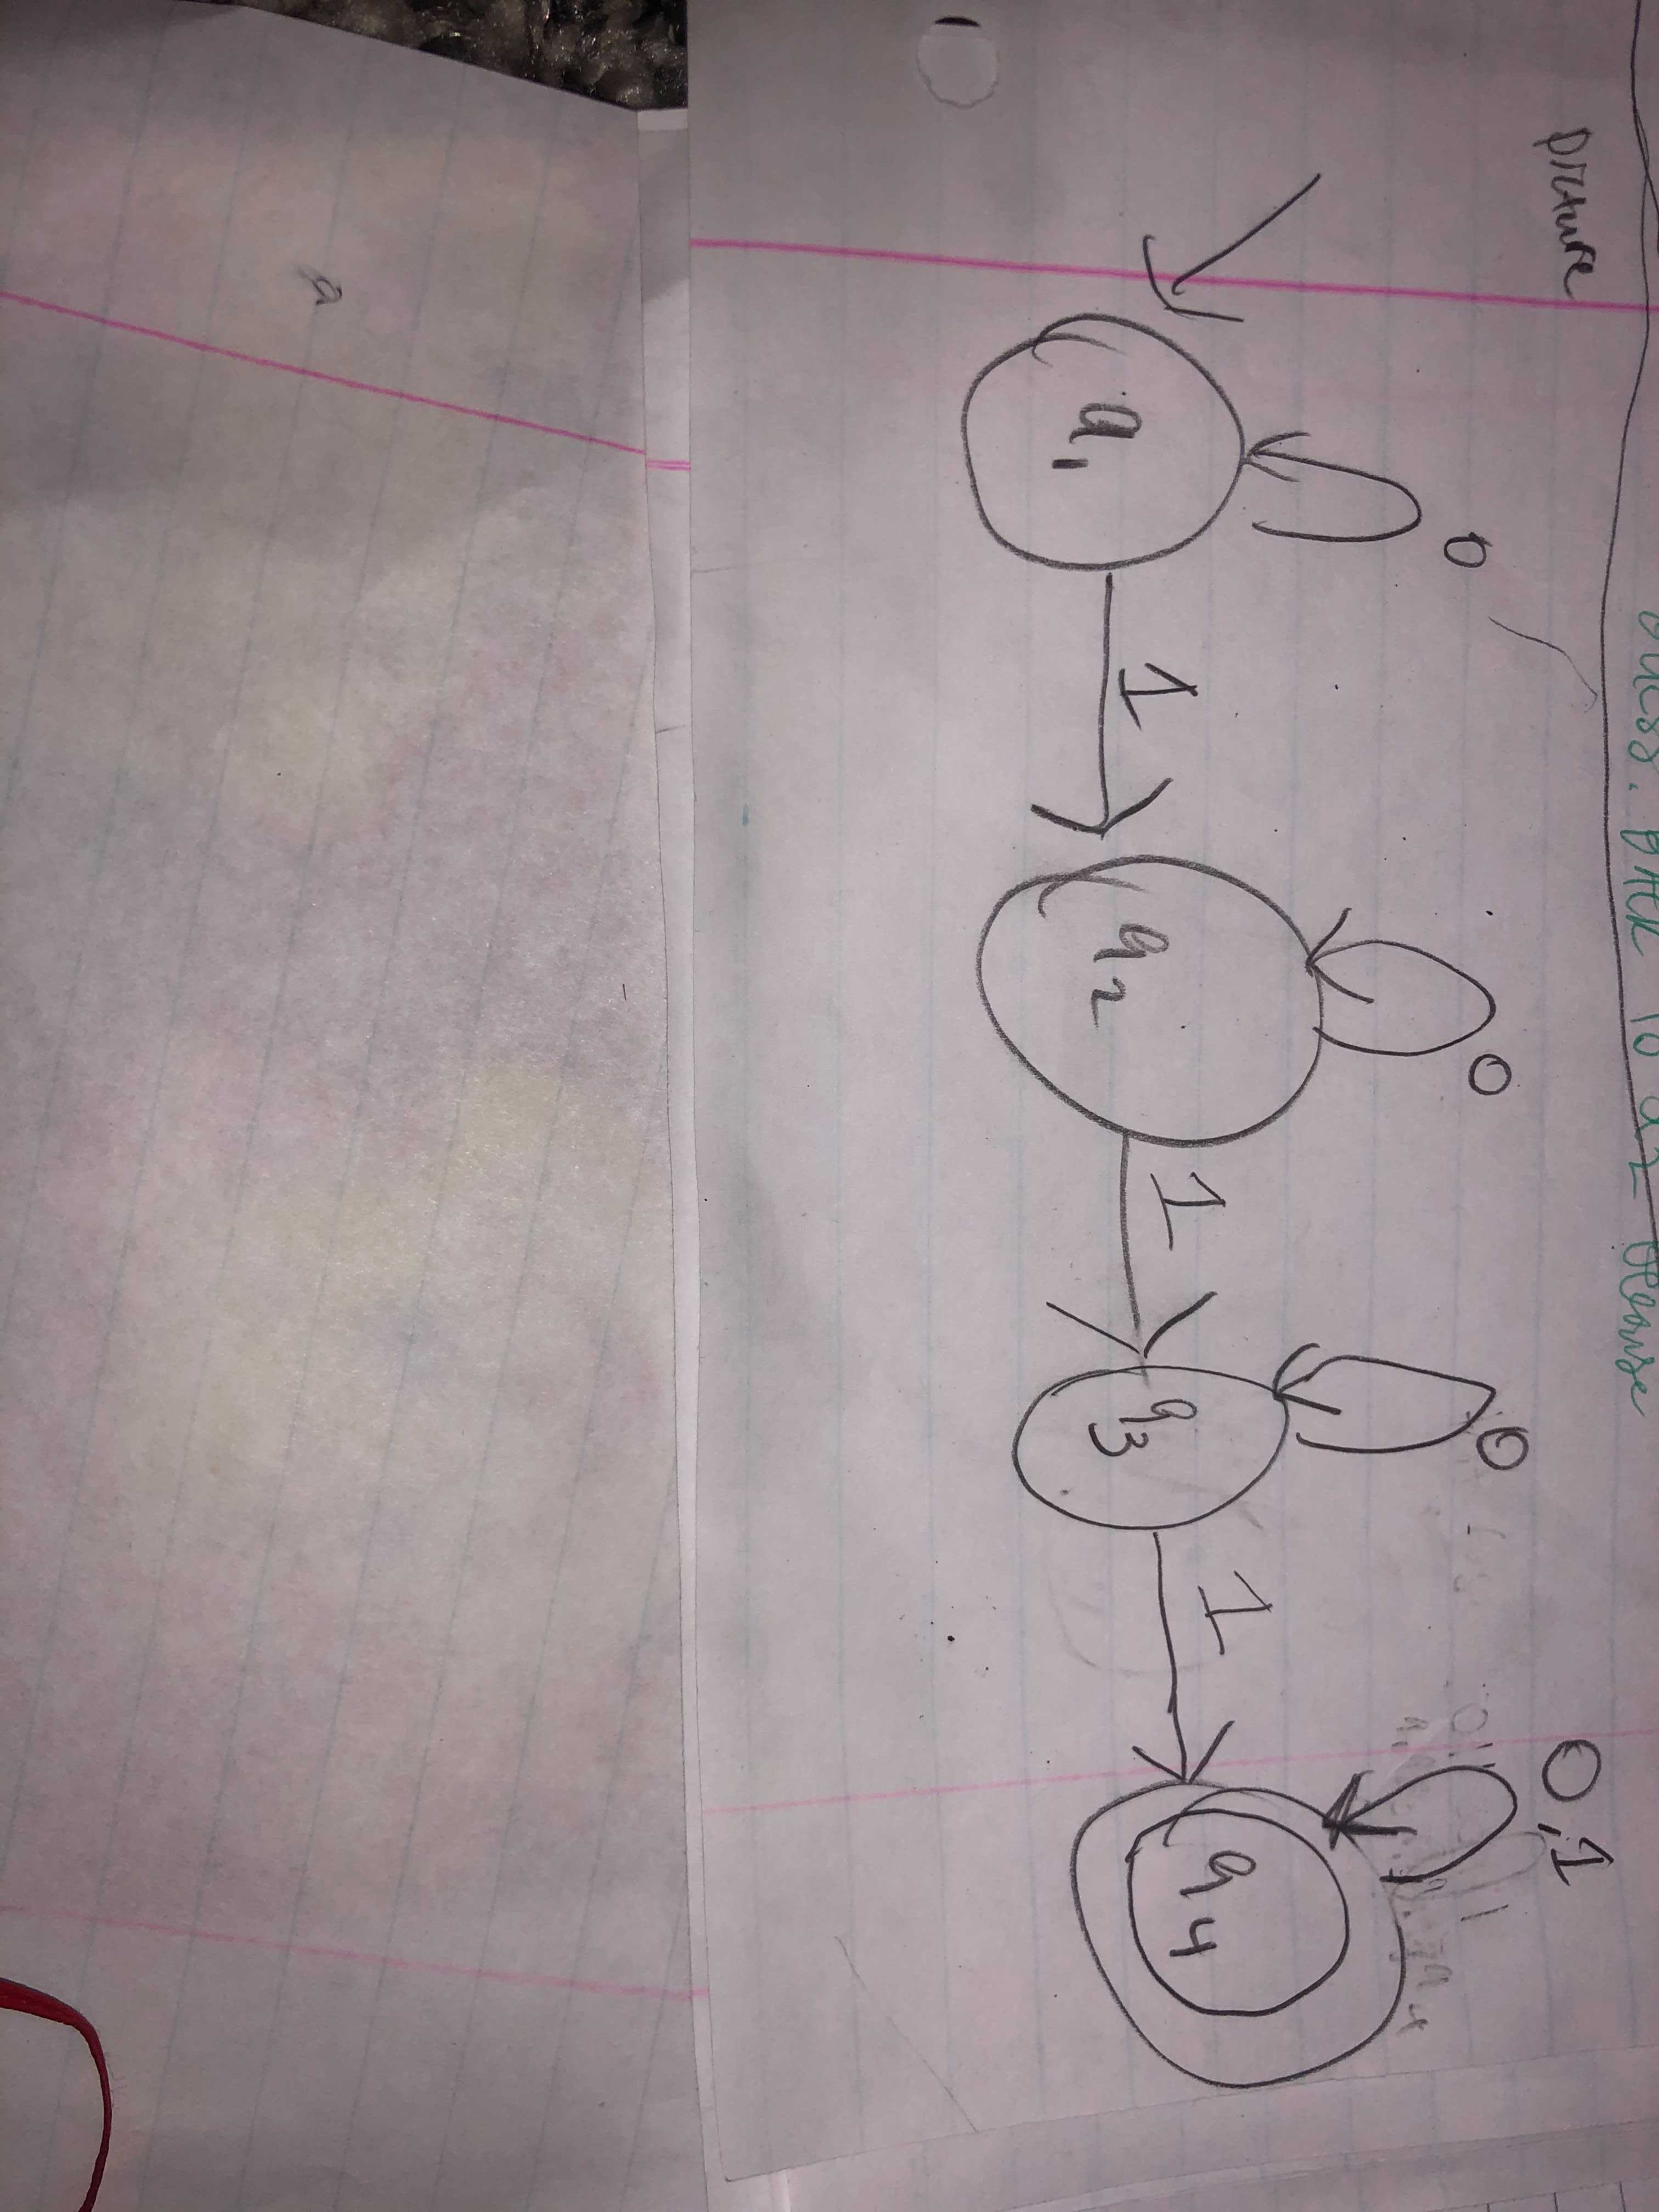
\includegraphics[angle=90,width=15cm,height=15cm,keepaspectratio]{pics/page3}

c.

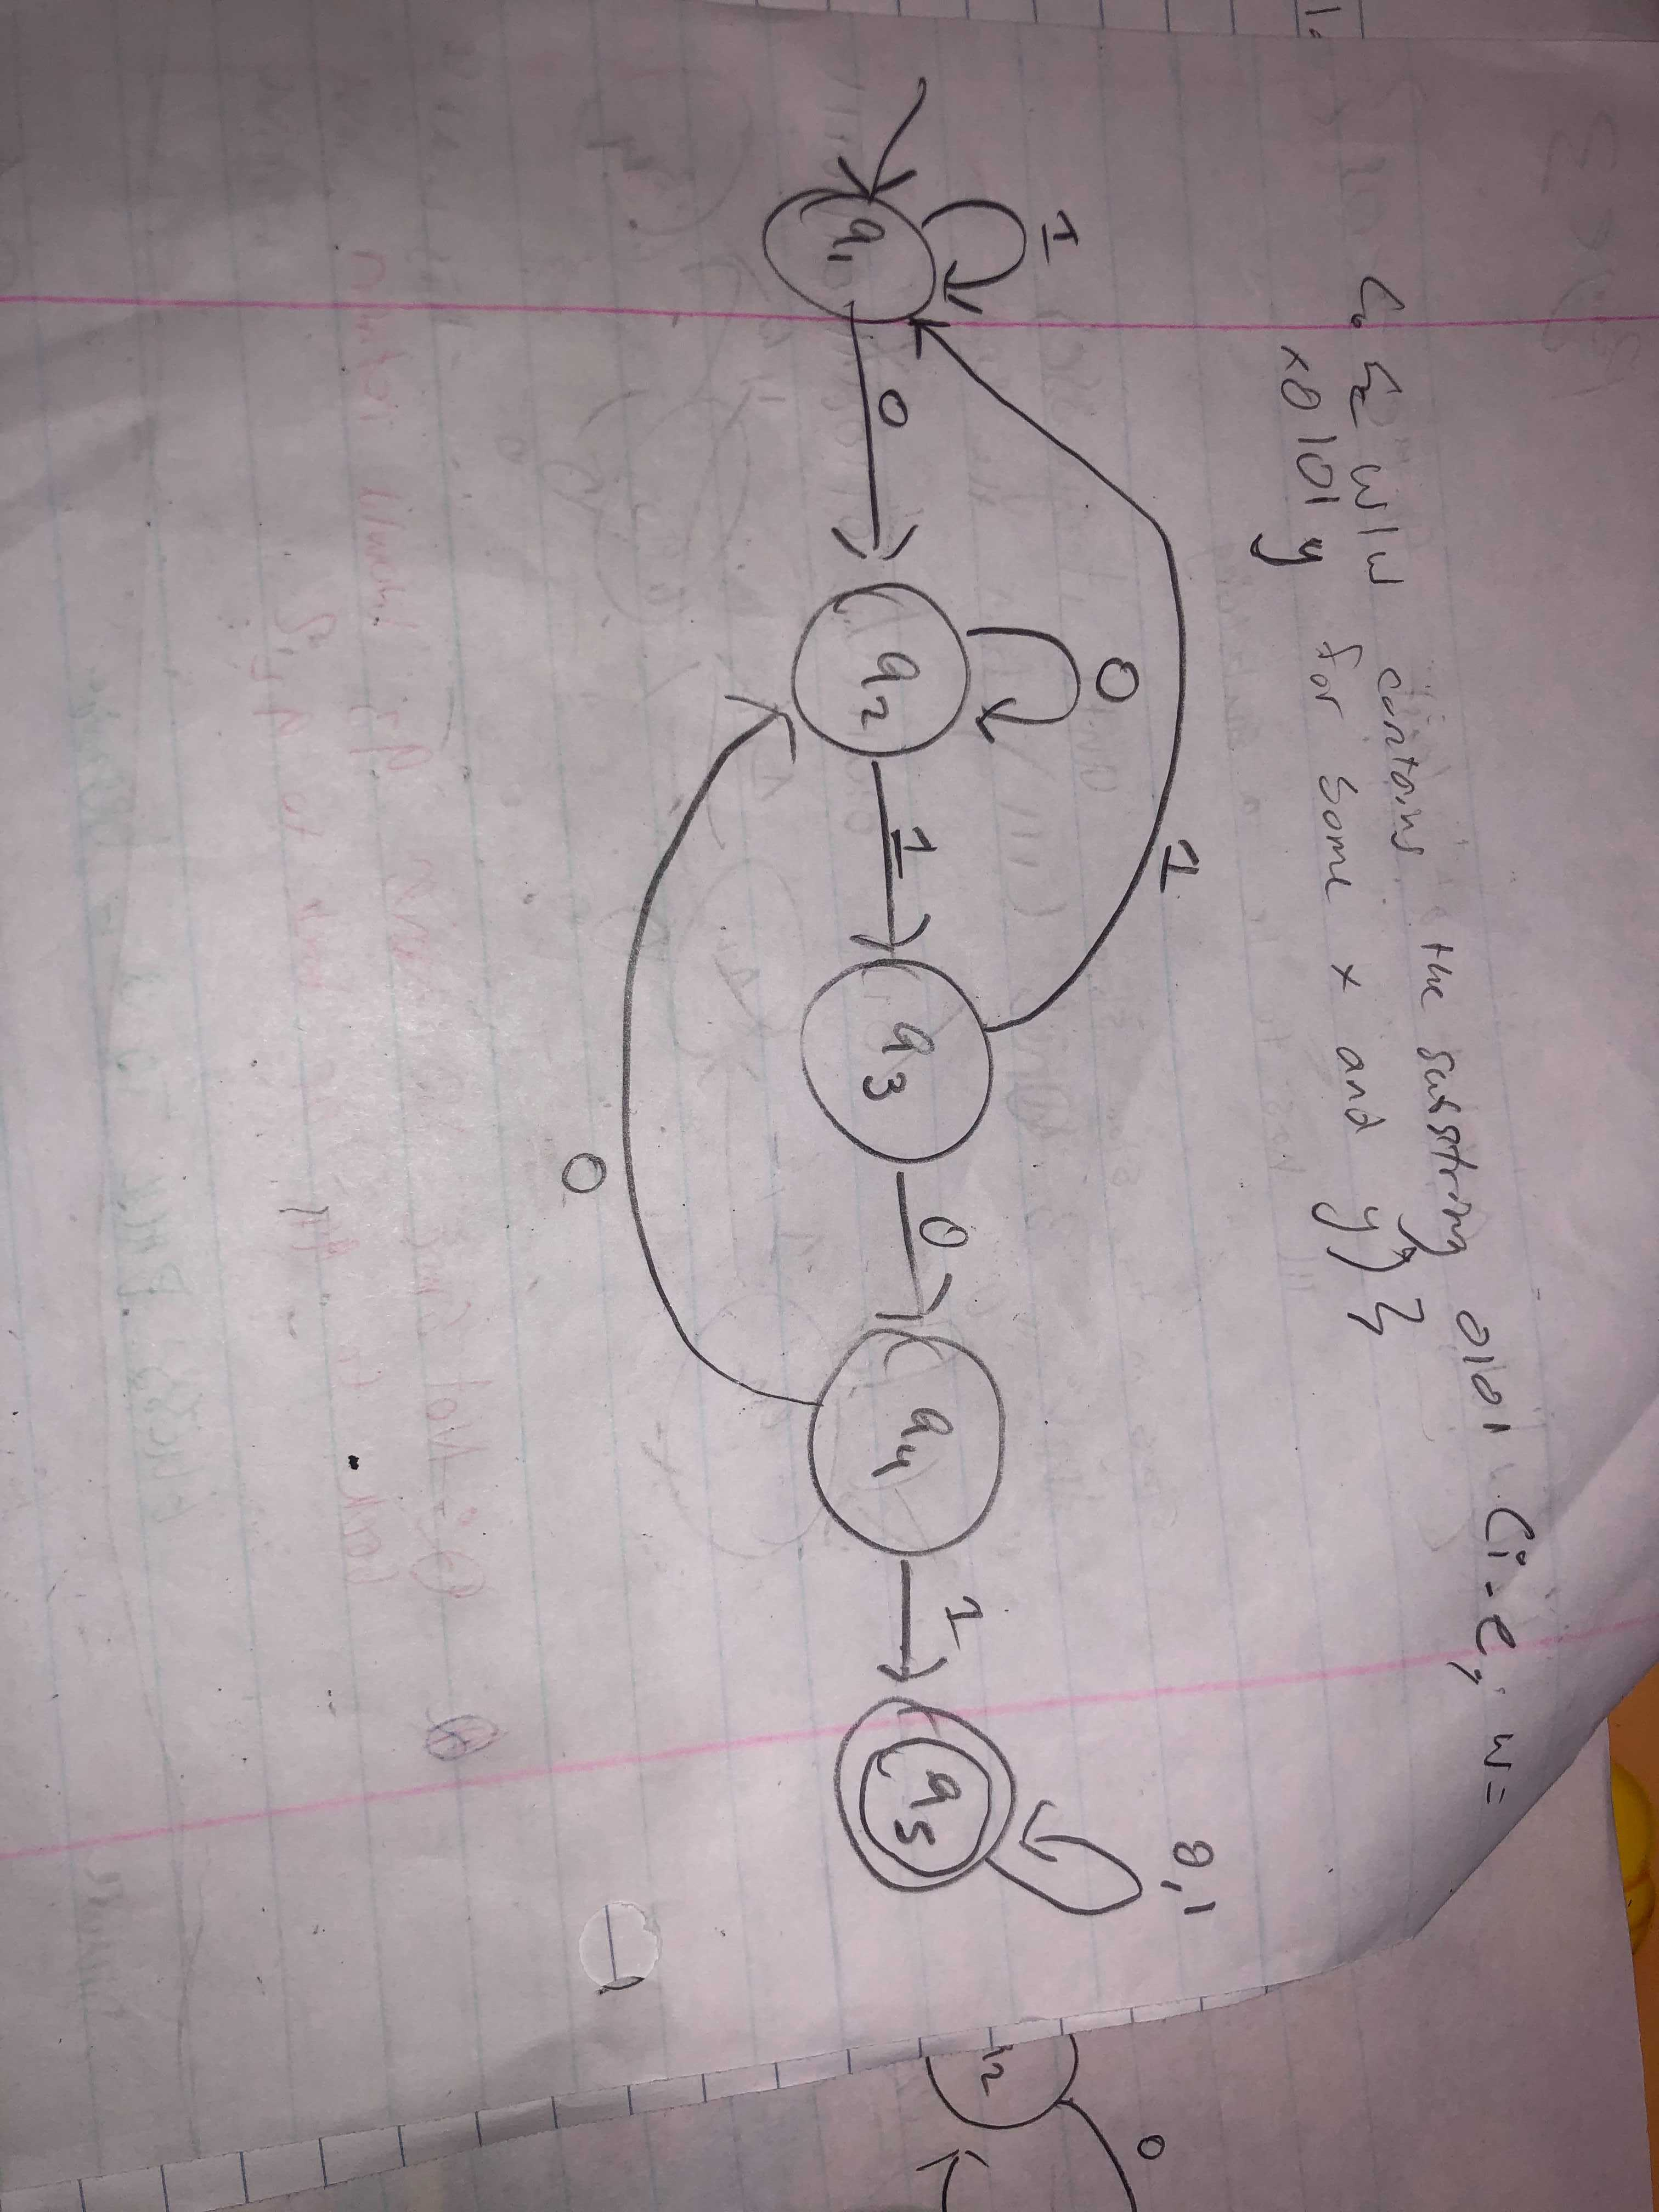
\includegraphics[angle=90,width=15cm,height=15cm,keepaspectratio]{pics/page4}

d.

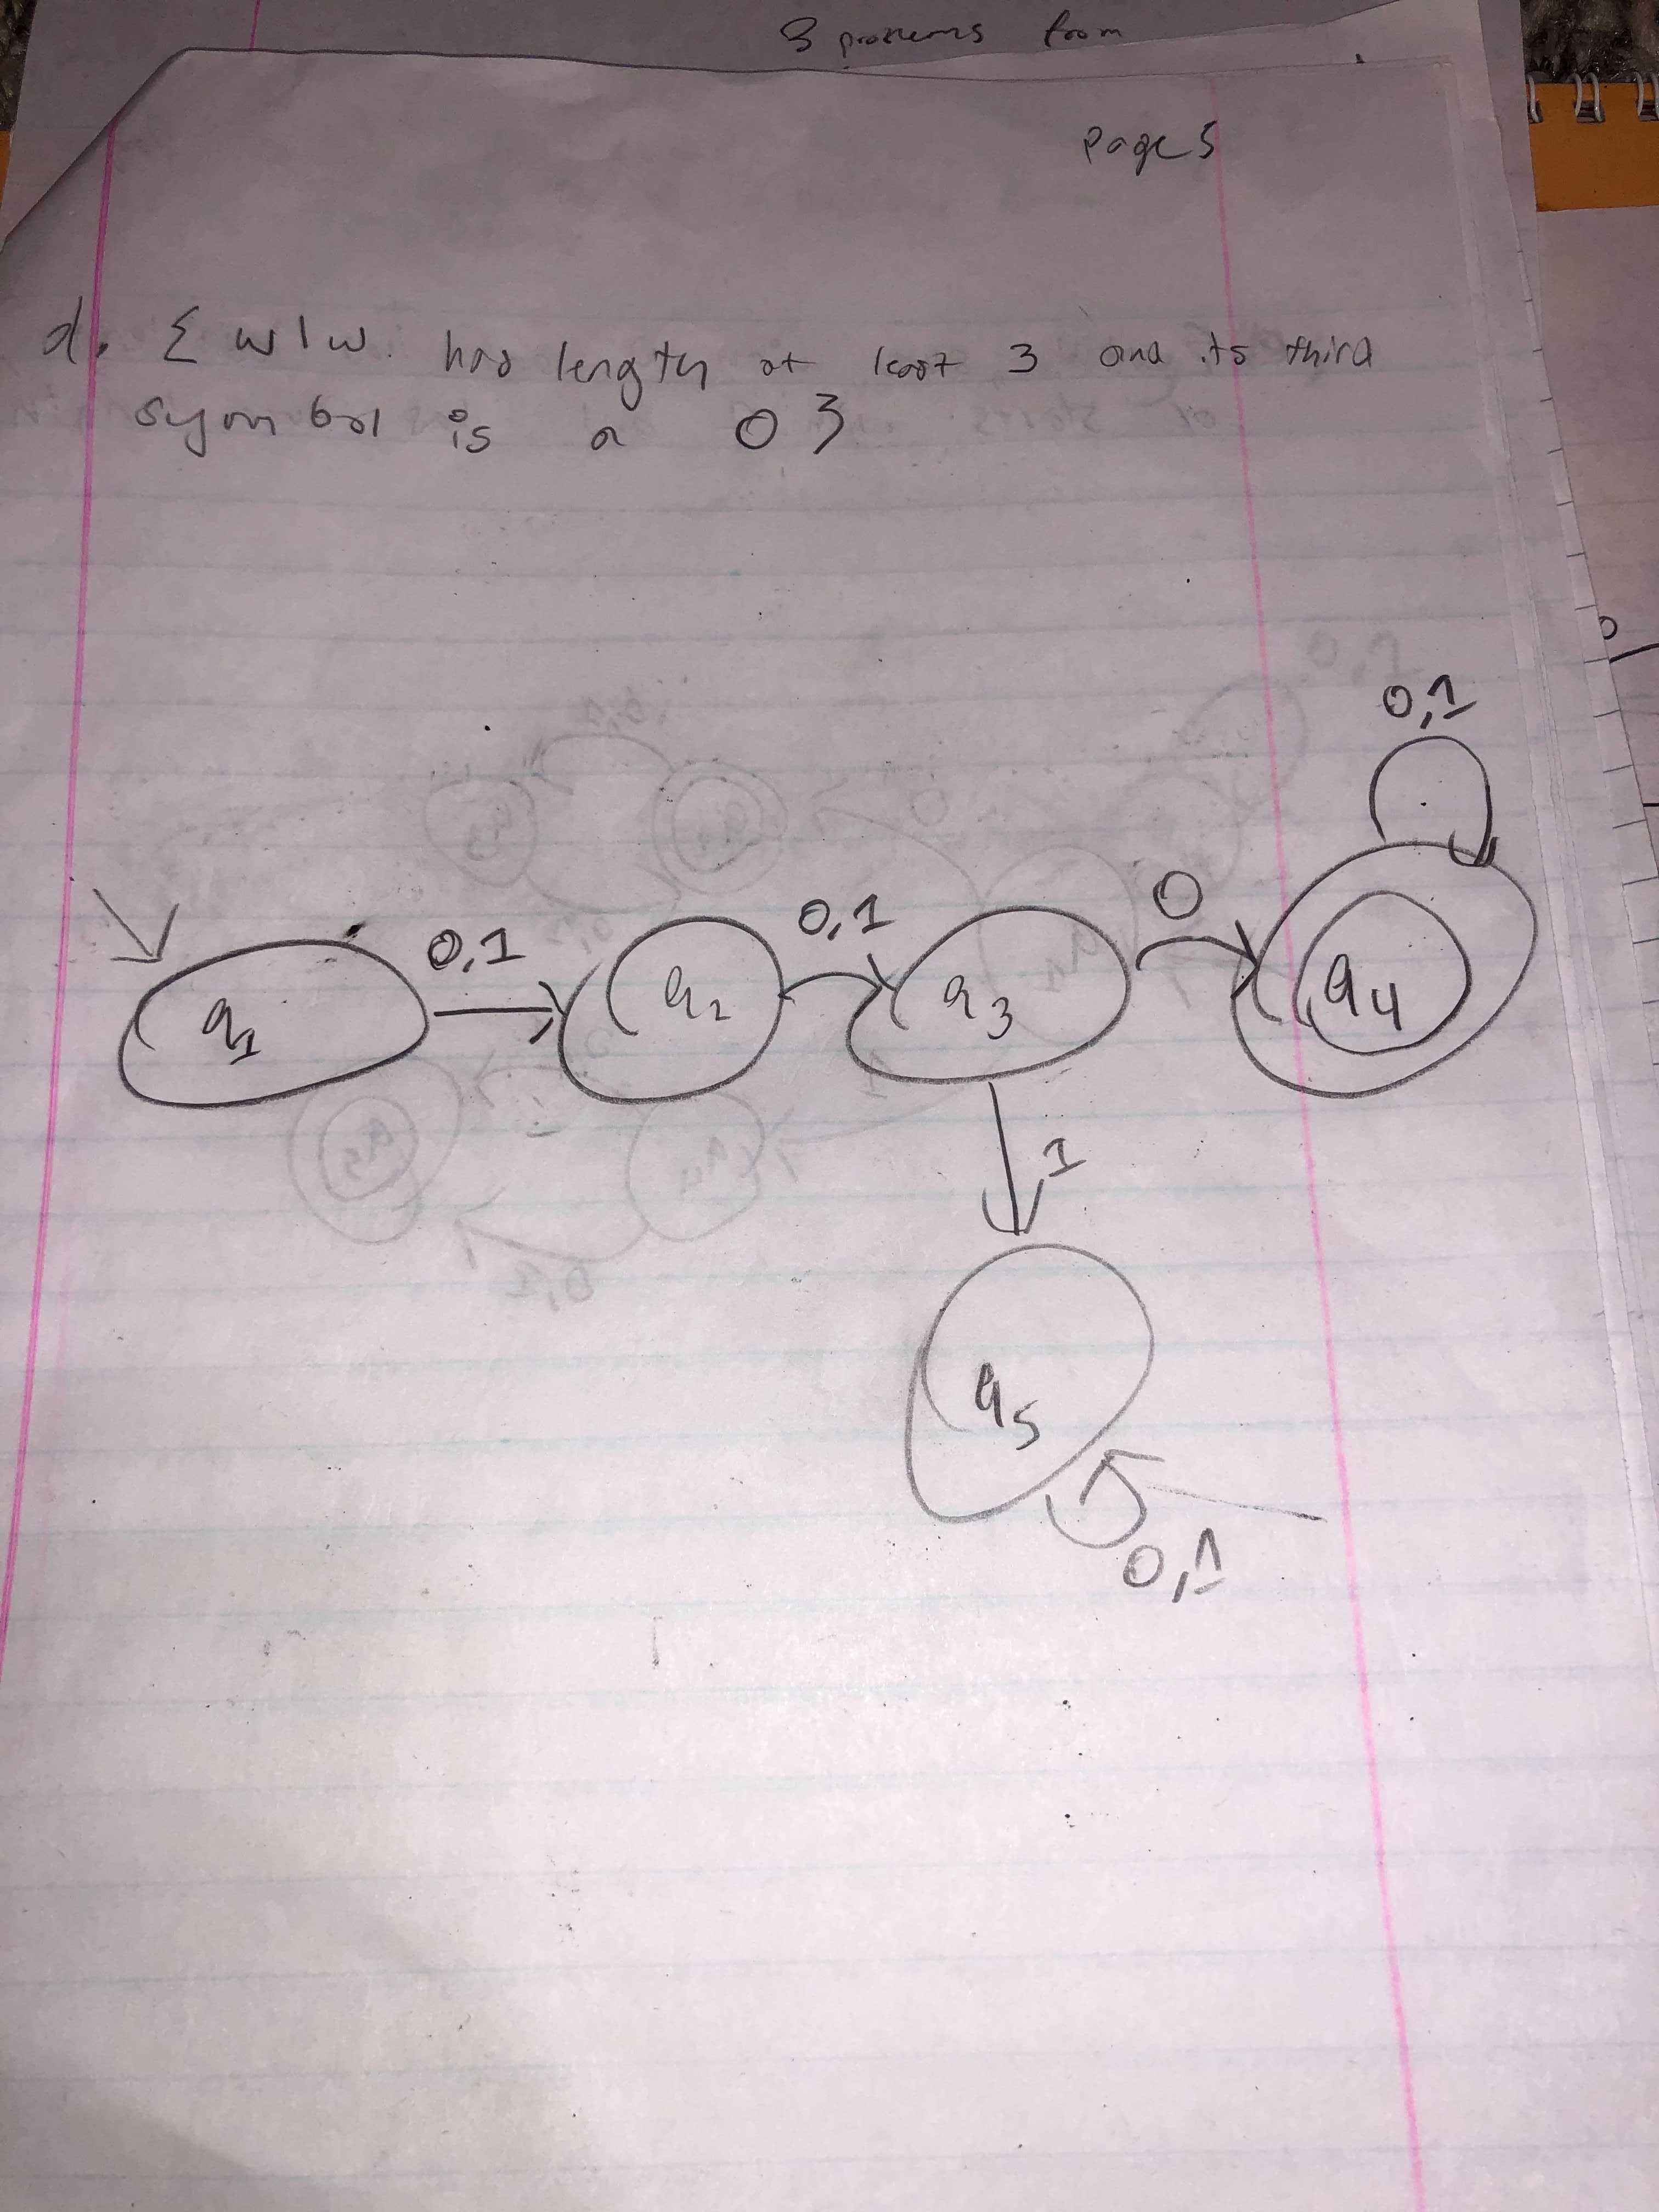
\includegraphics[width=15cm,height=15cm,keepaspectratio]{pics/page5}

e.

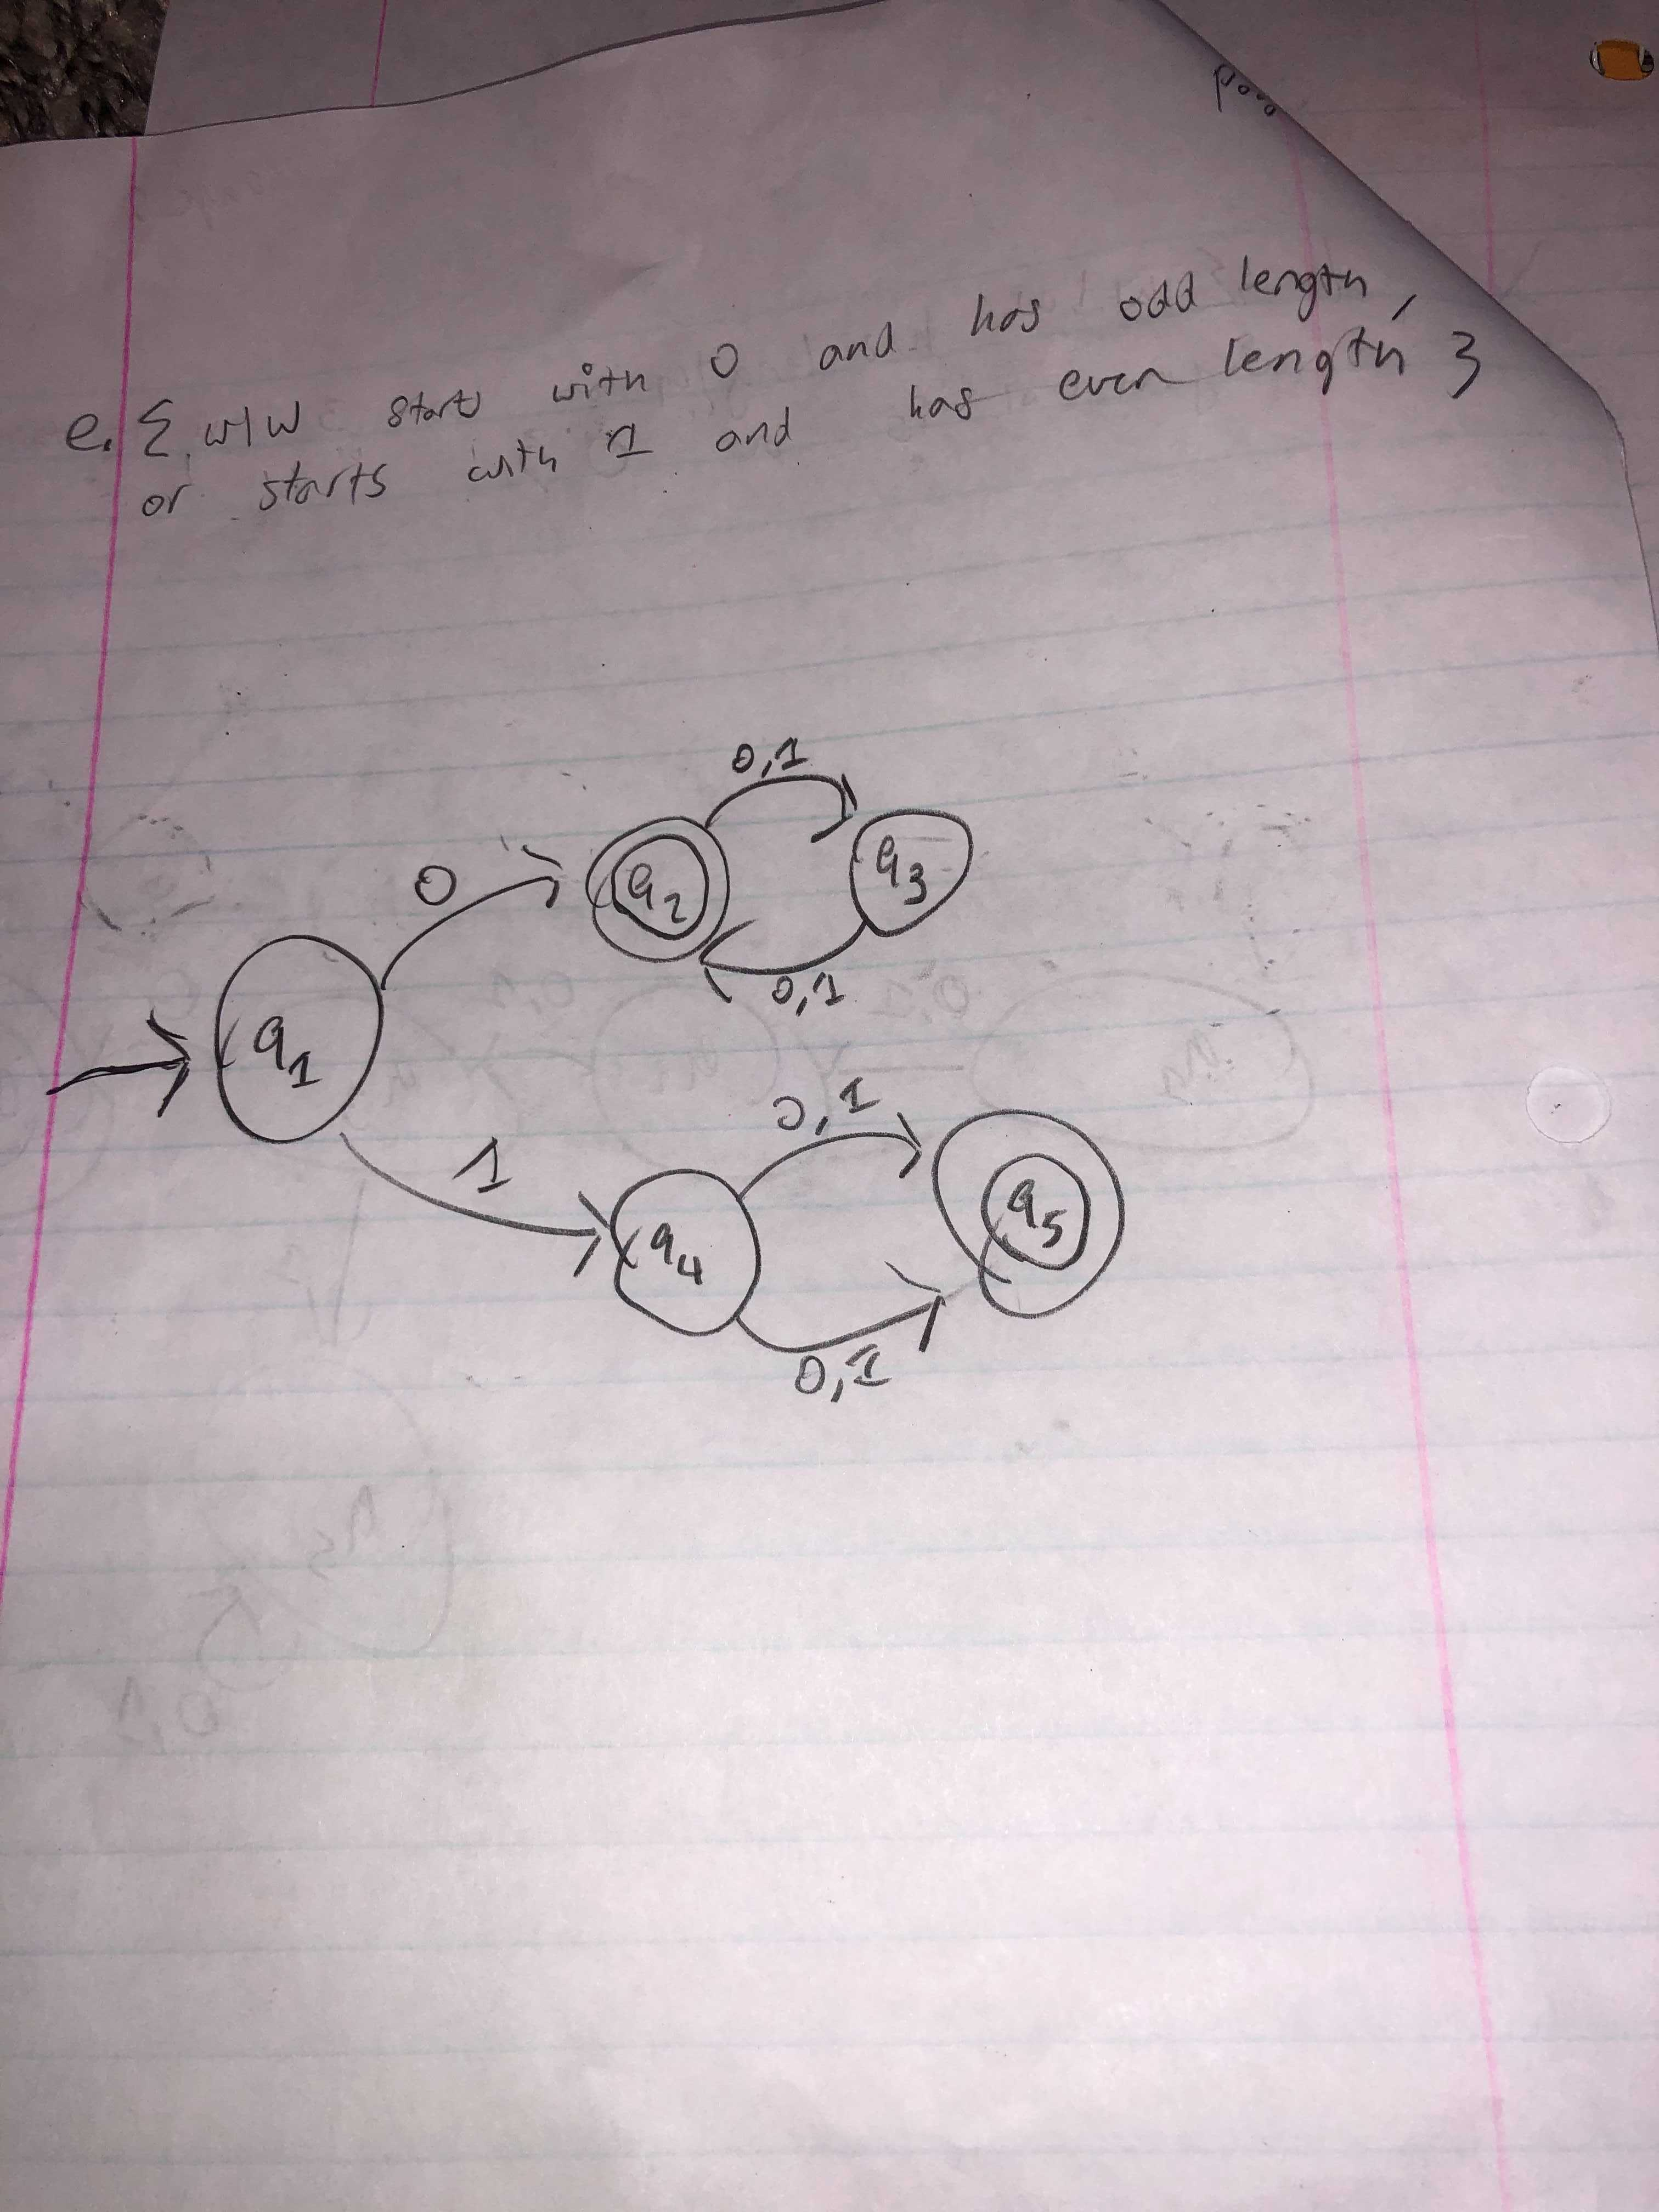
\includegraphics[width=15cm,height=15cm,keepaspectratio]{pics/page6}

f.

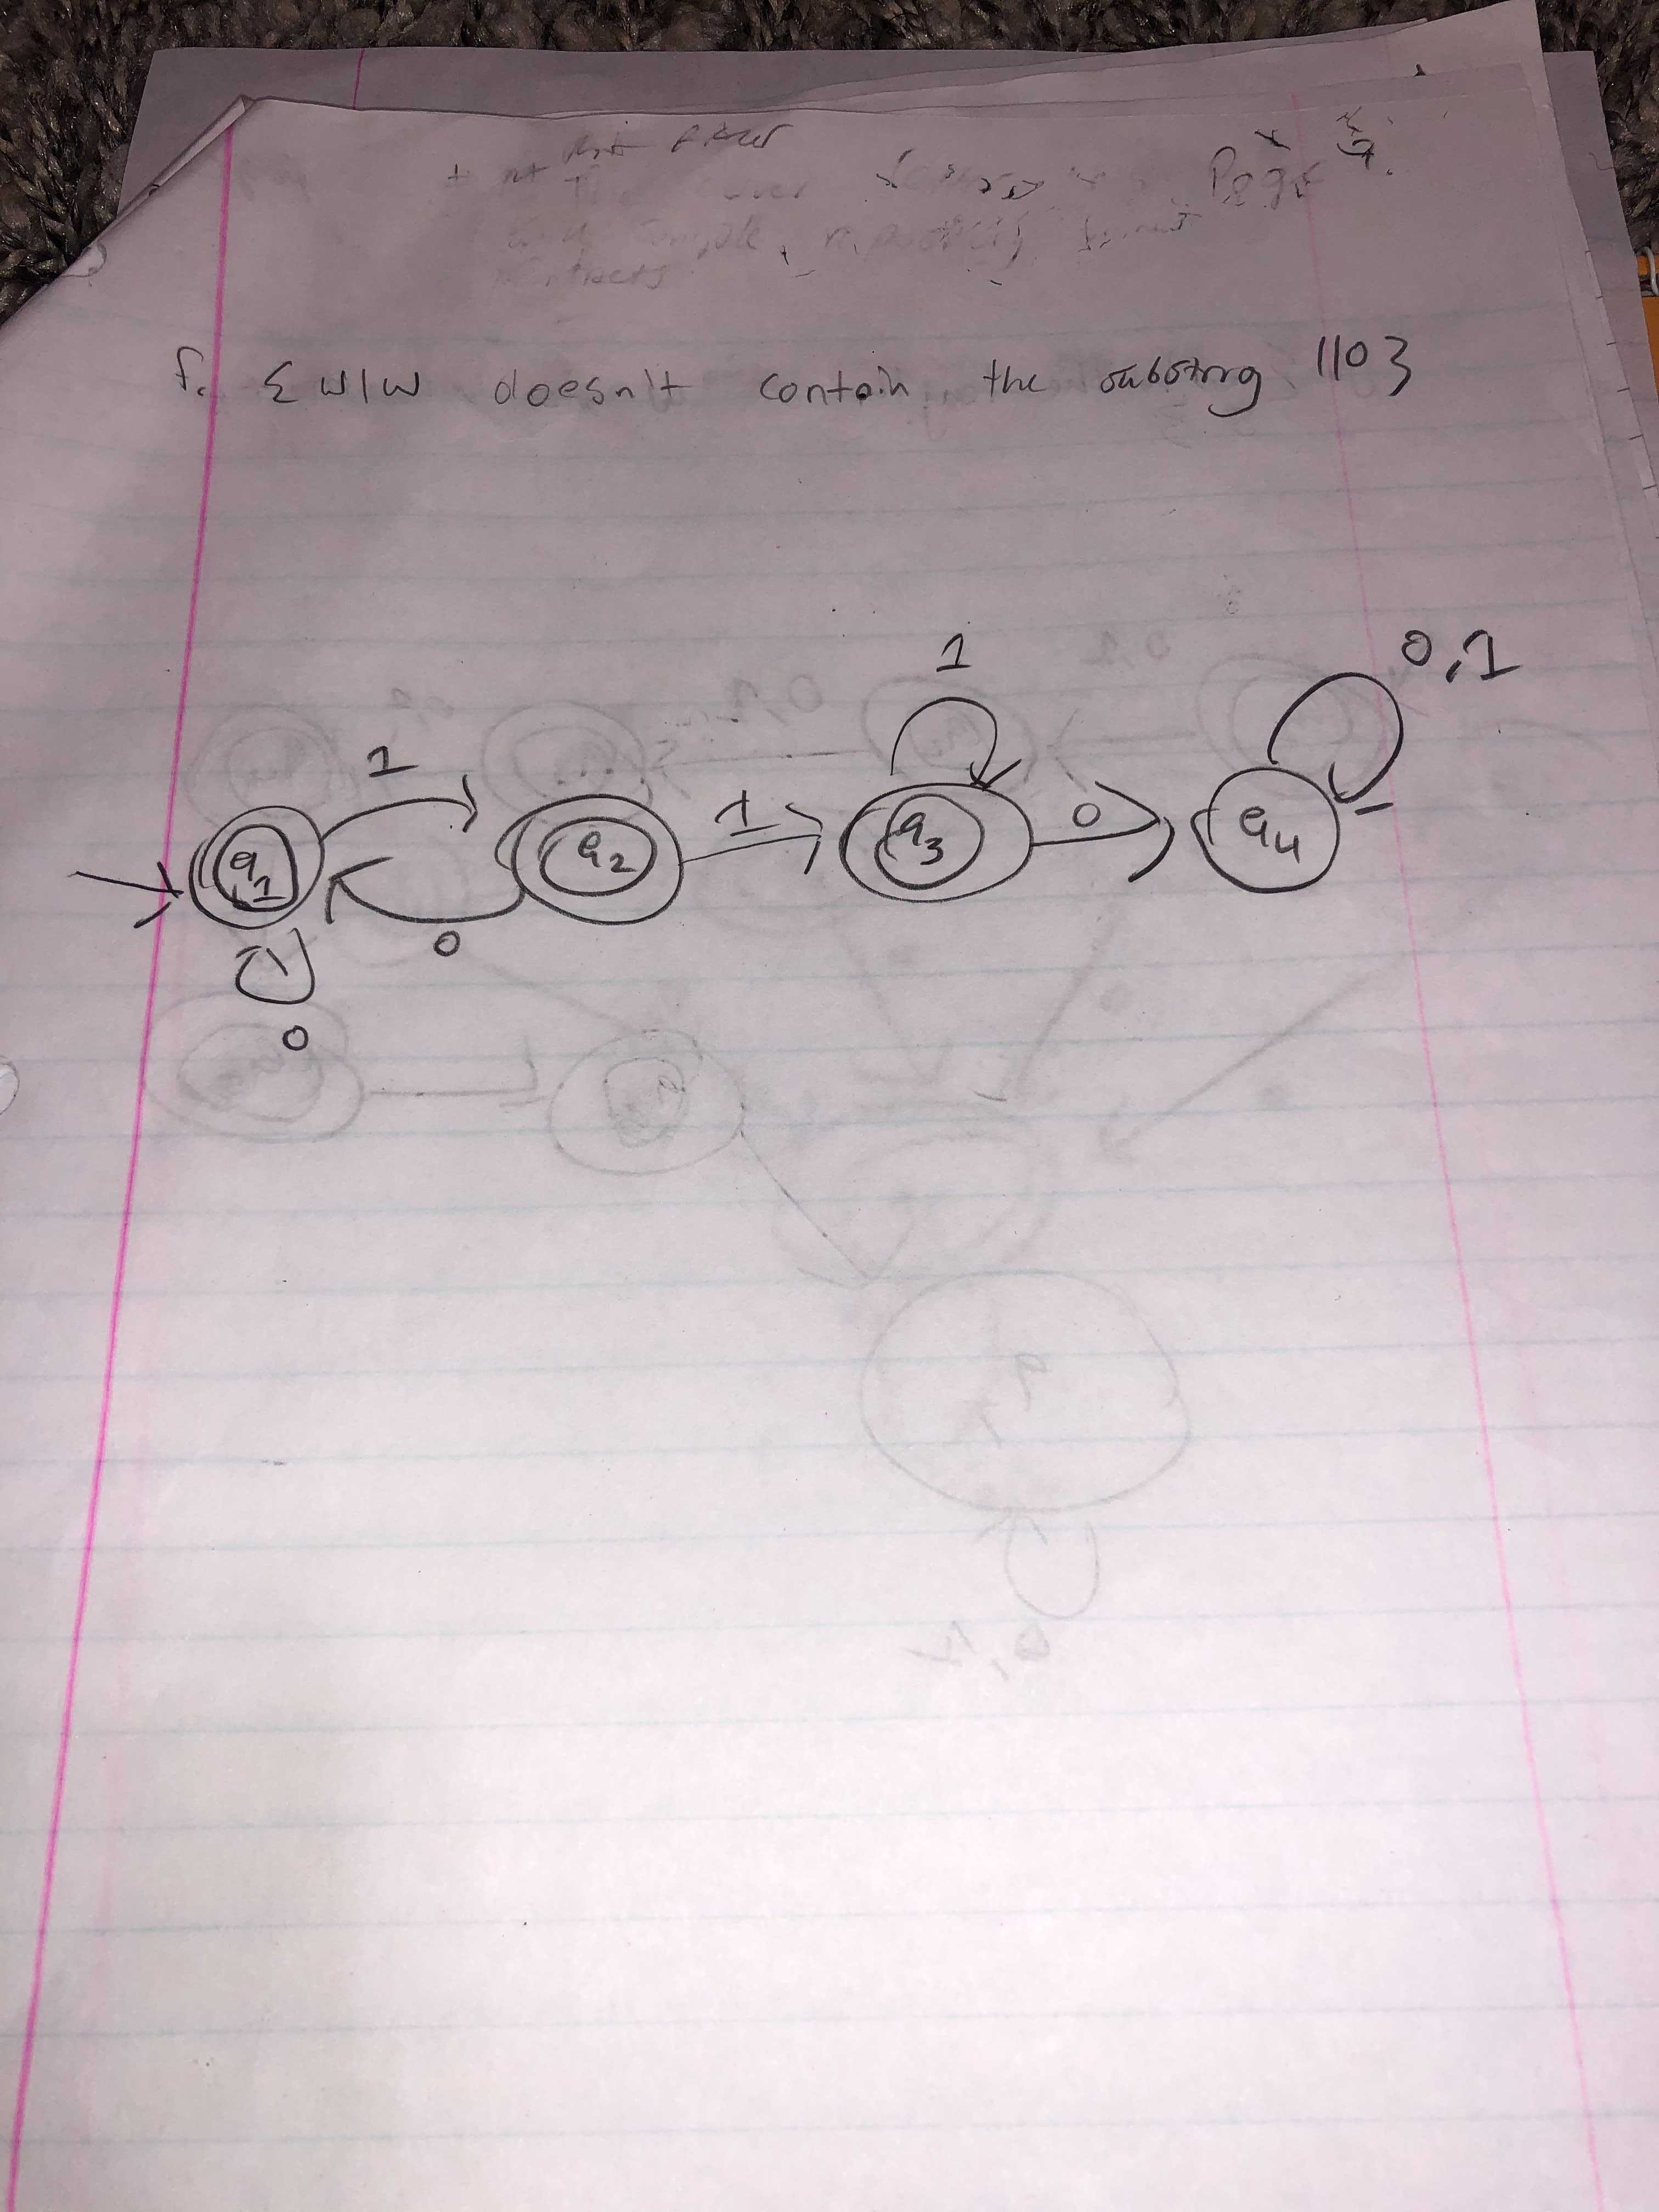
\includegraphics[width=15cm,height=15cm,keepaspectratio]{pics/page7}

g.

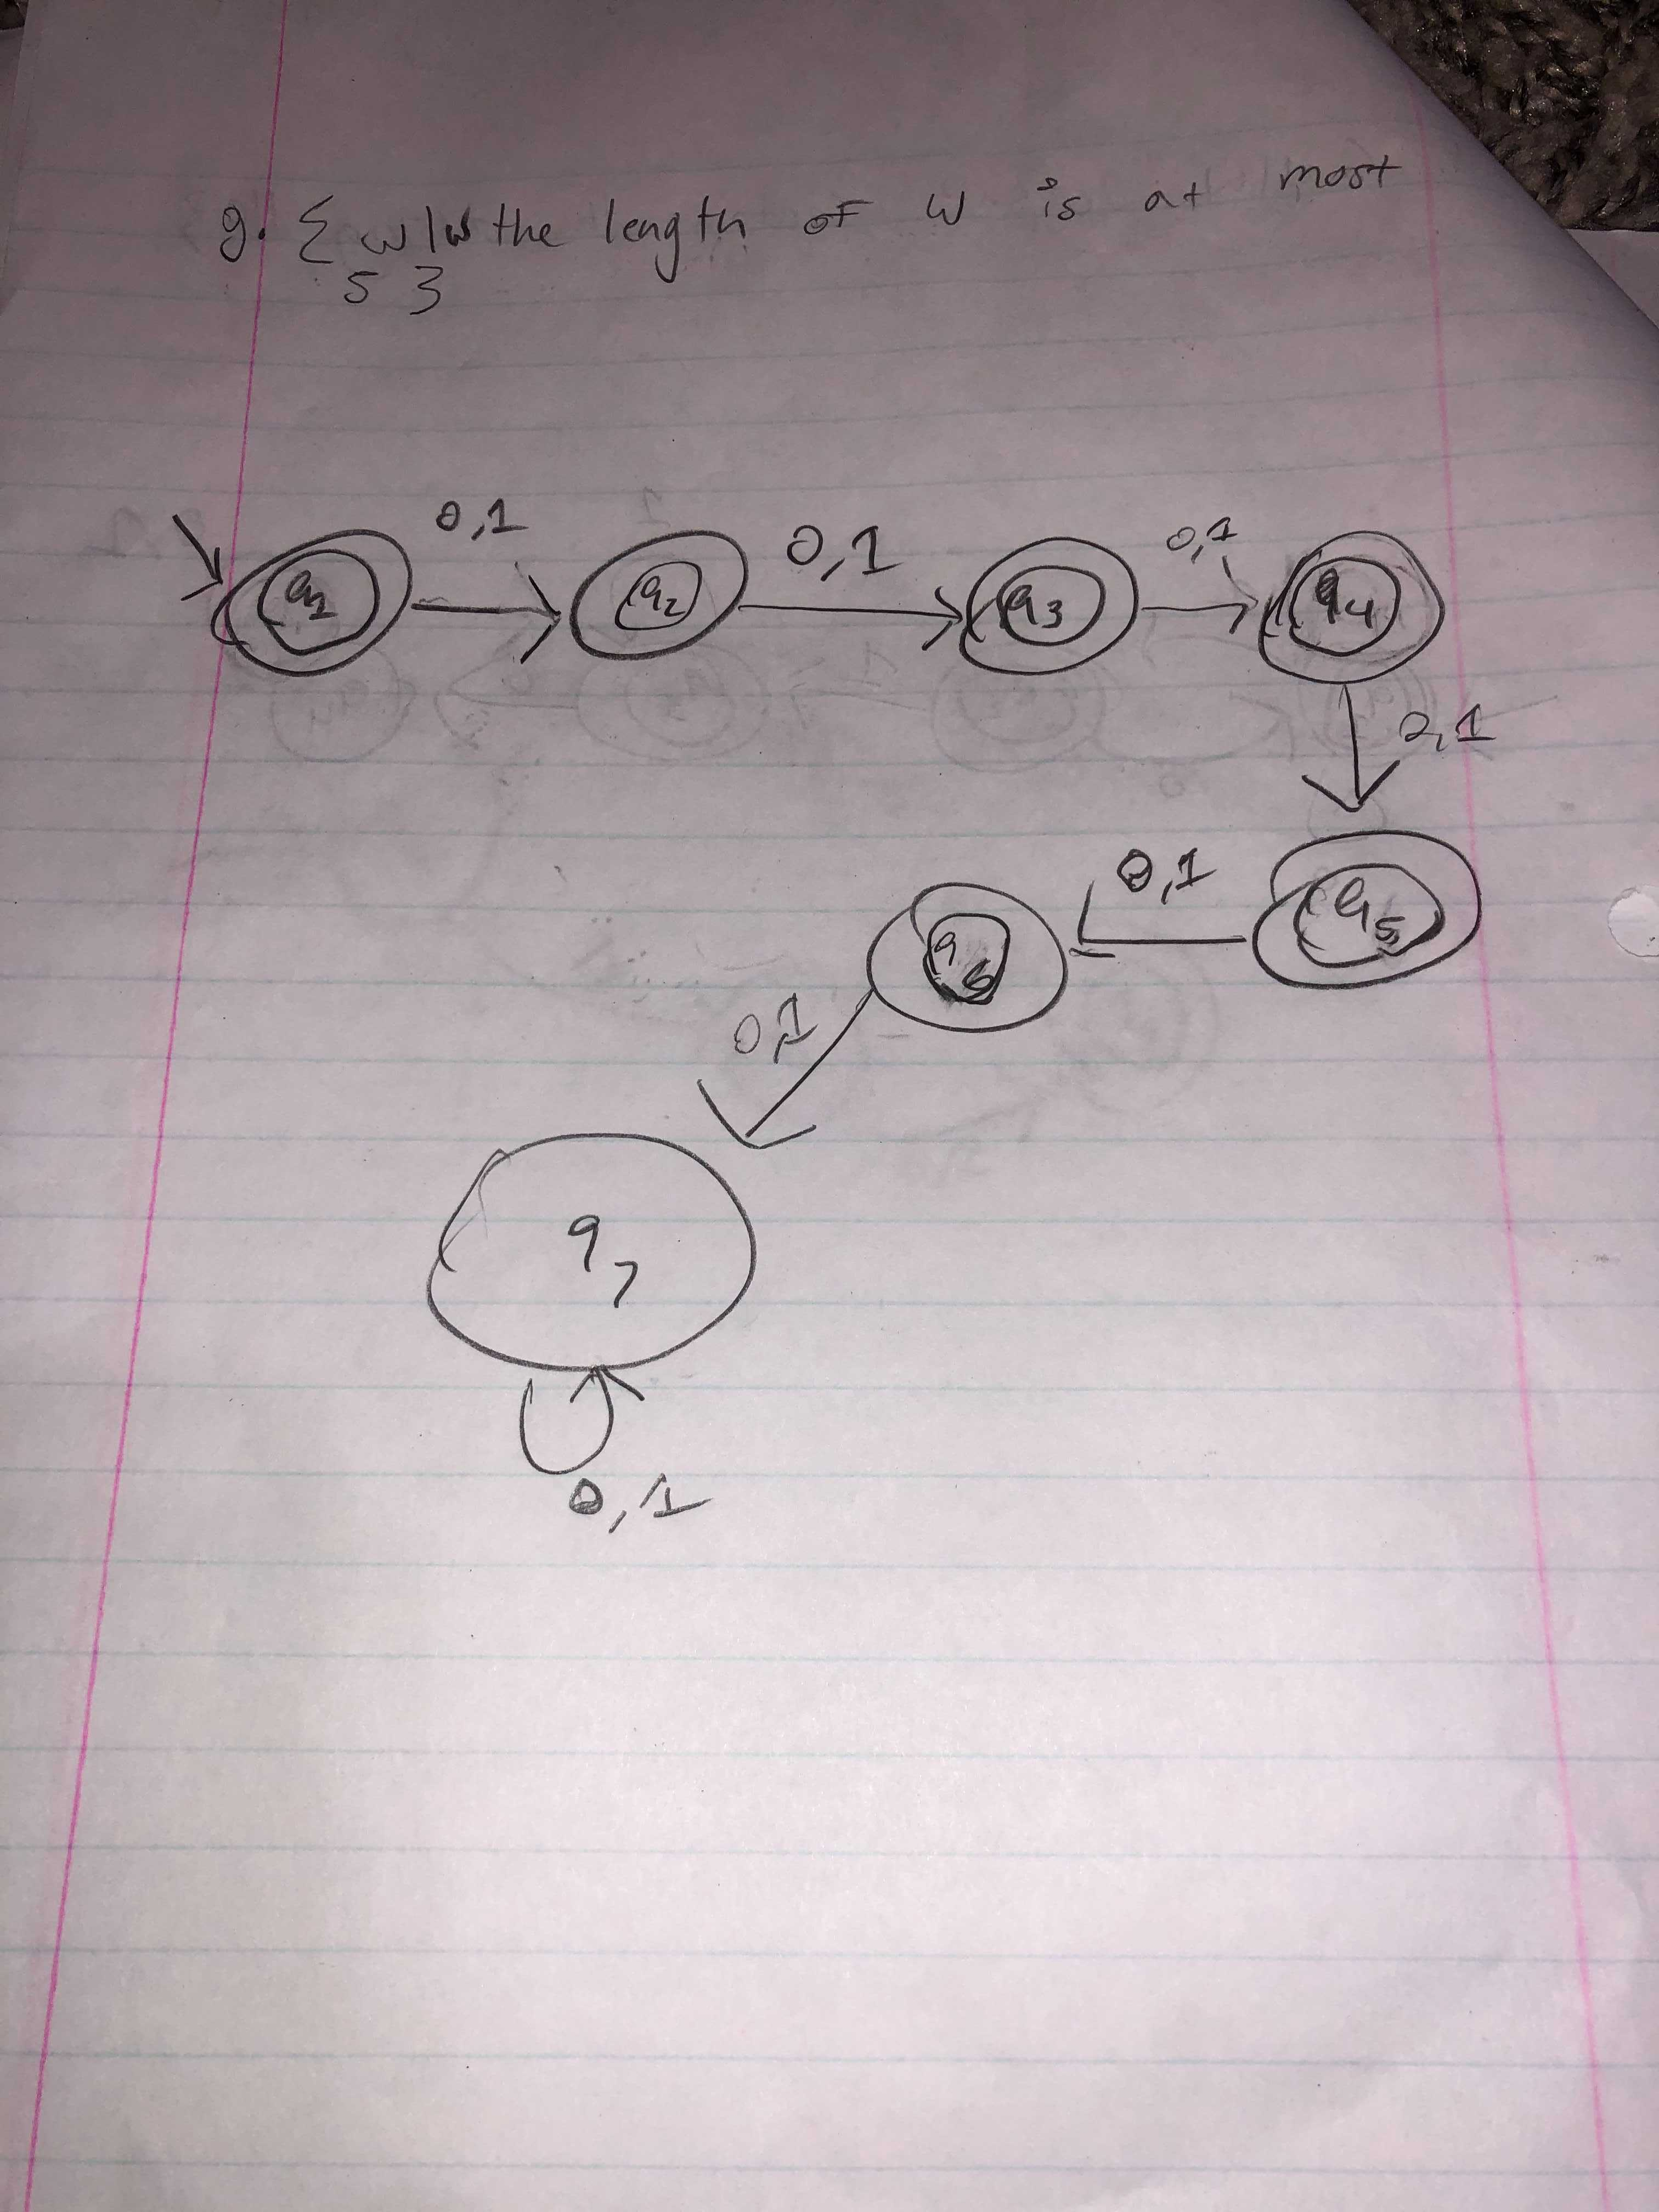
\includegraphics[width=15cm,height=15cm,keepaspectratio]{pics/page8}

h.

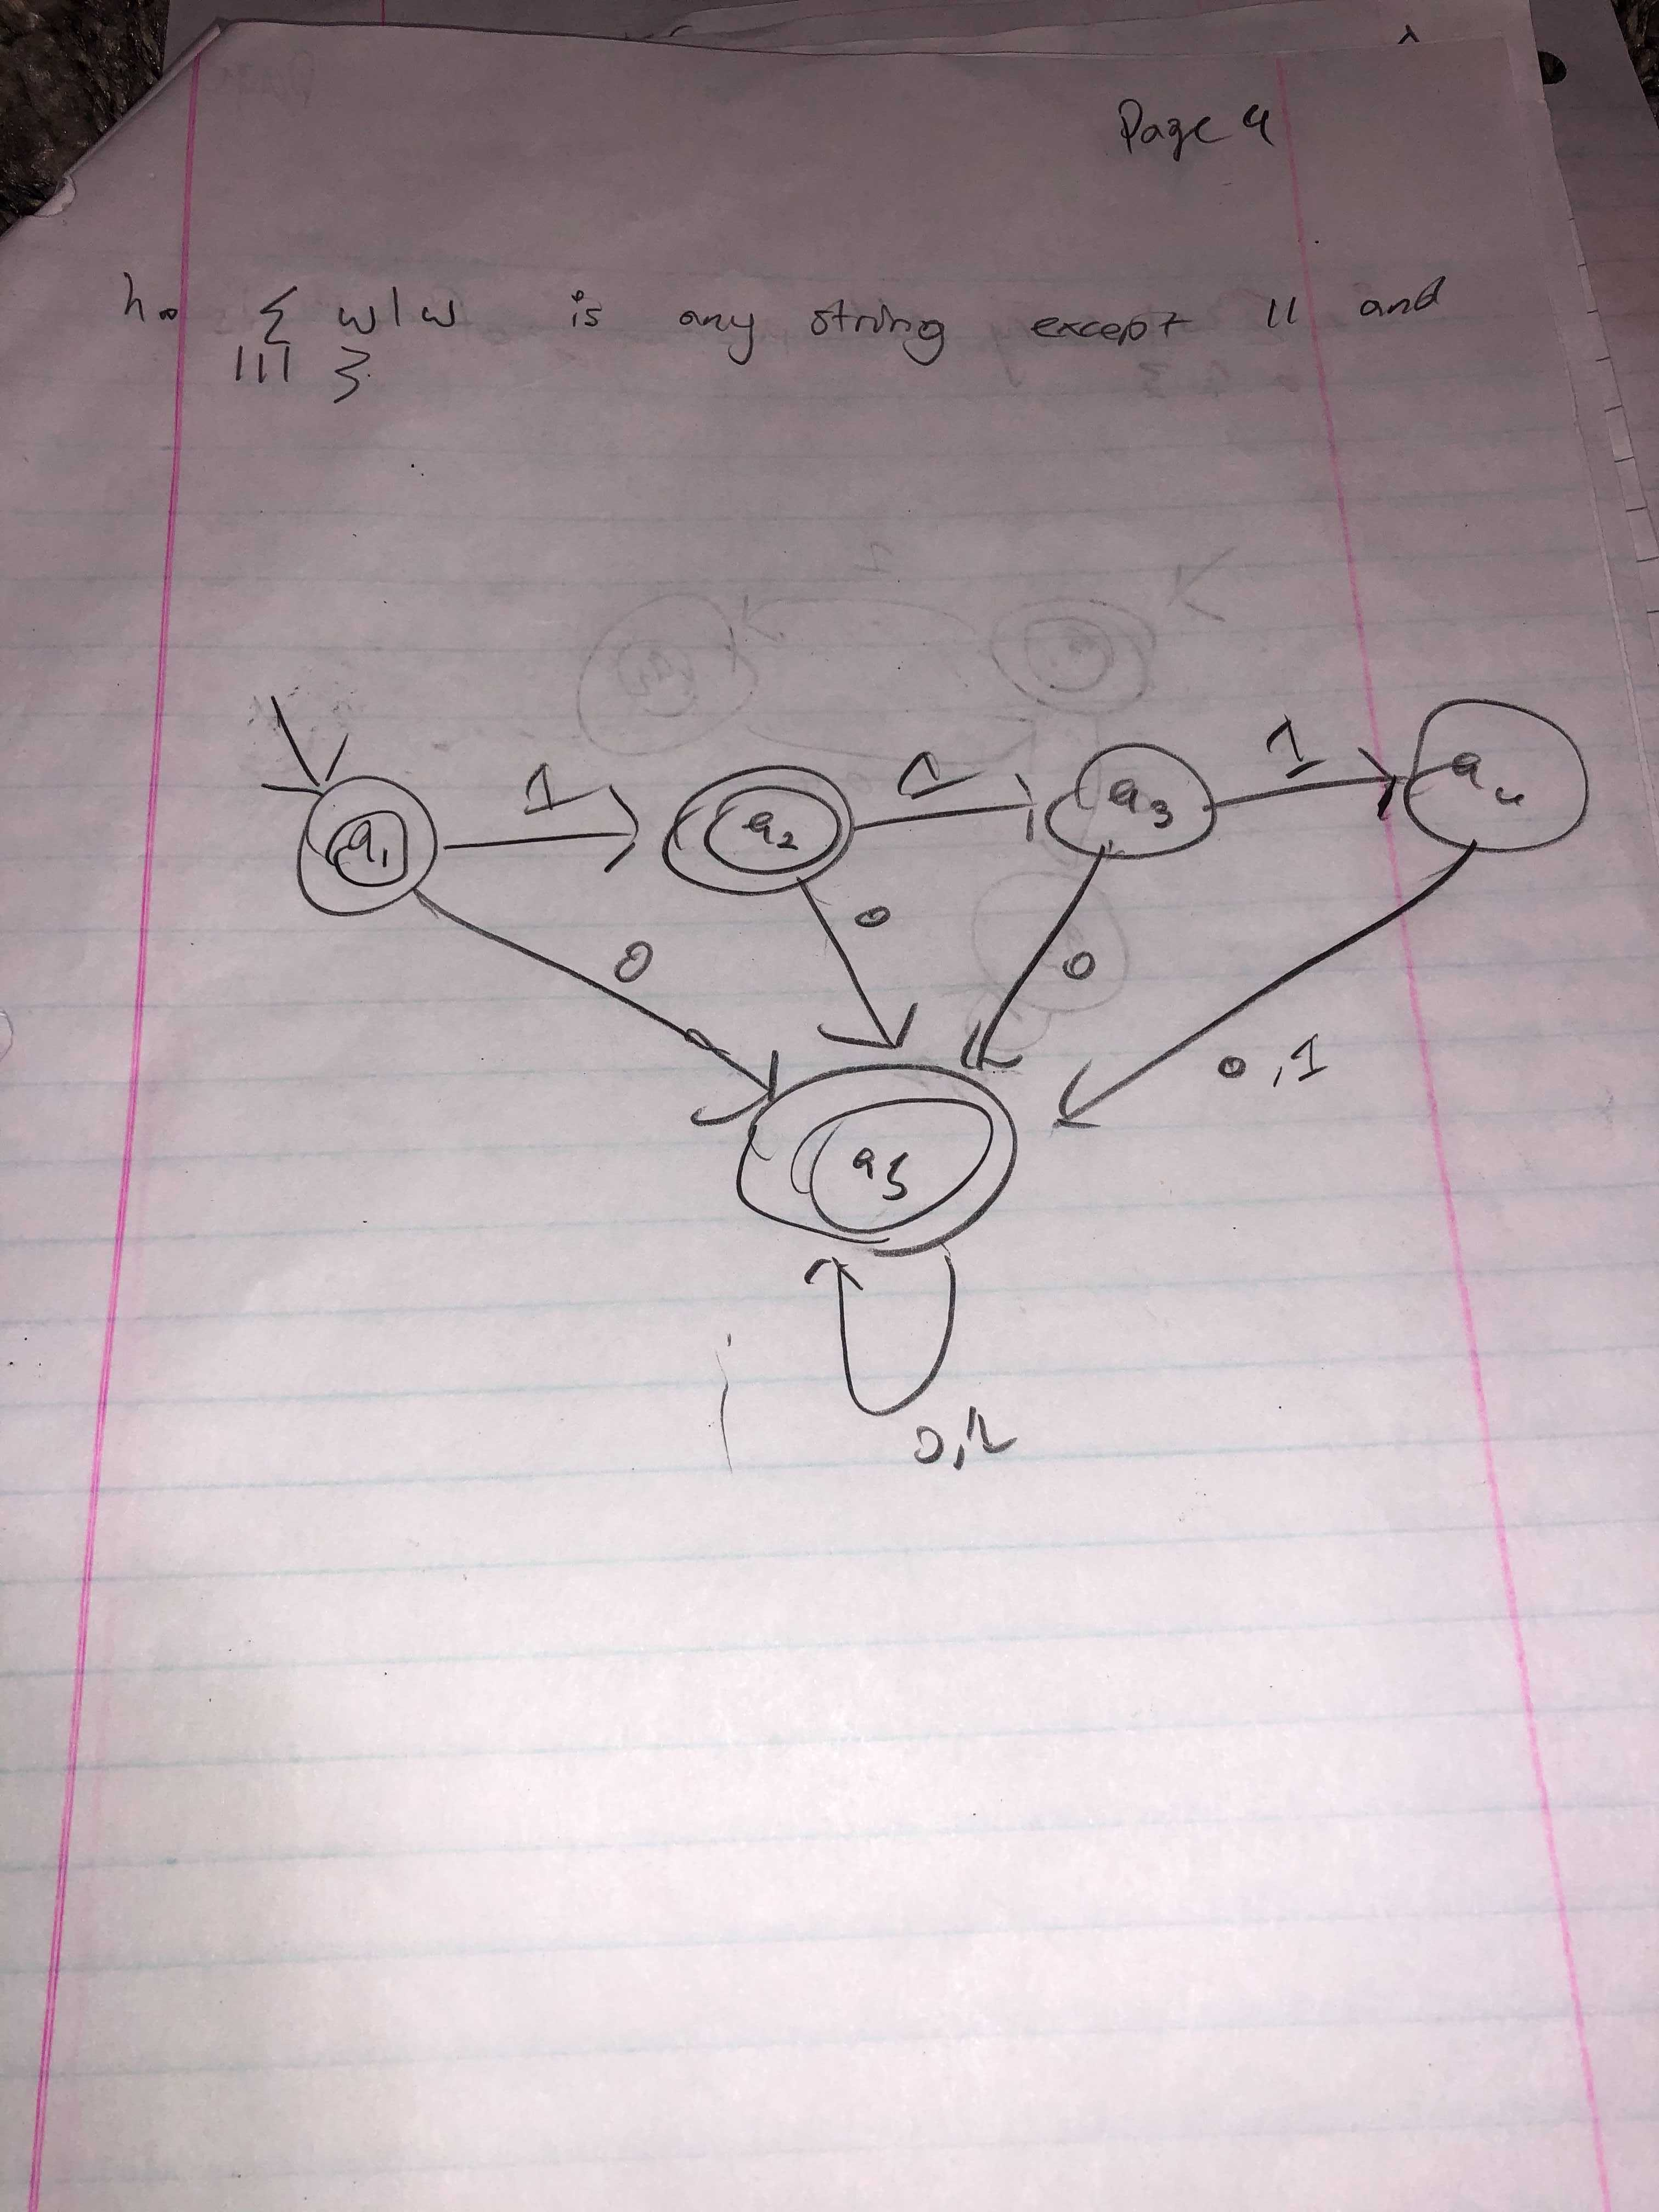
\includegraphics[width=15cm,height=15cm,keepaspectratio]{pics/page9}

i.

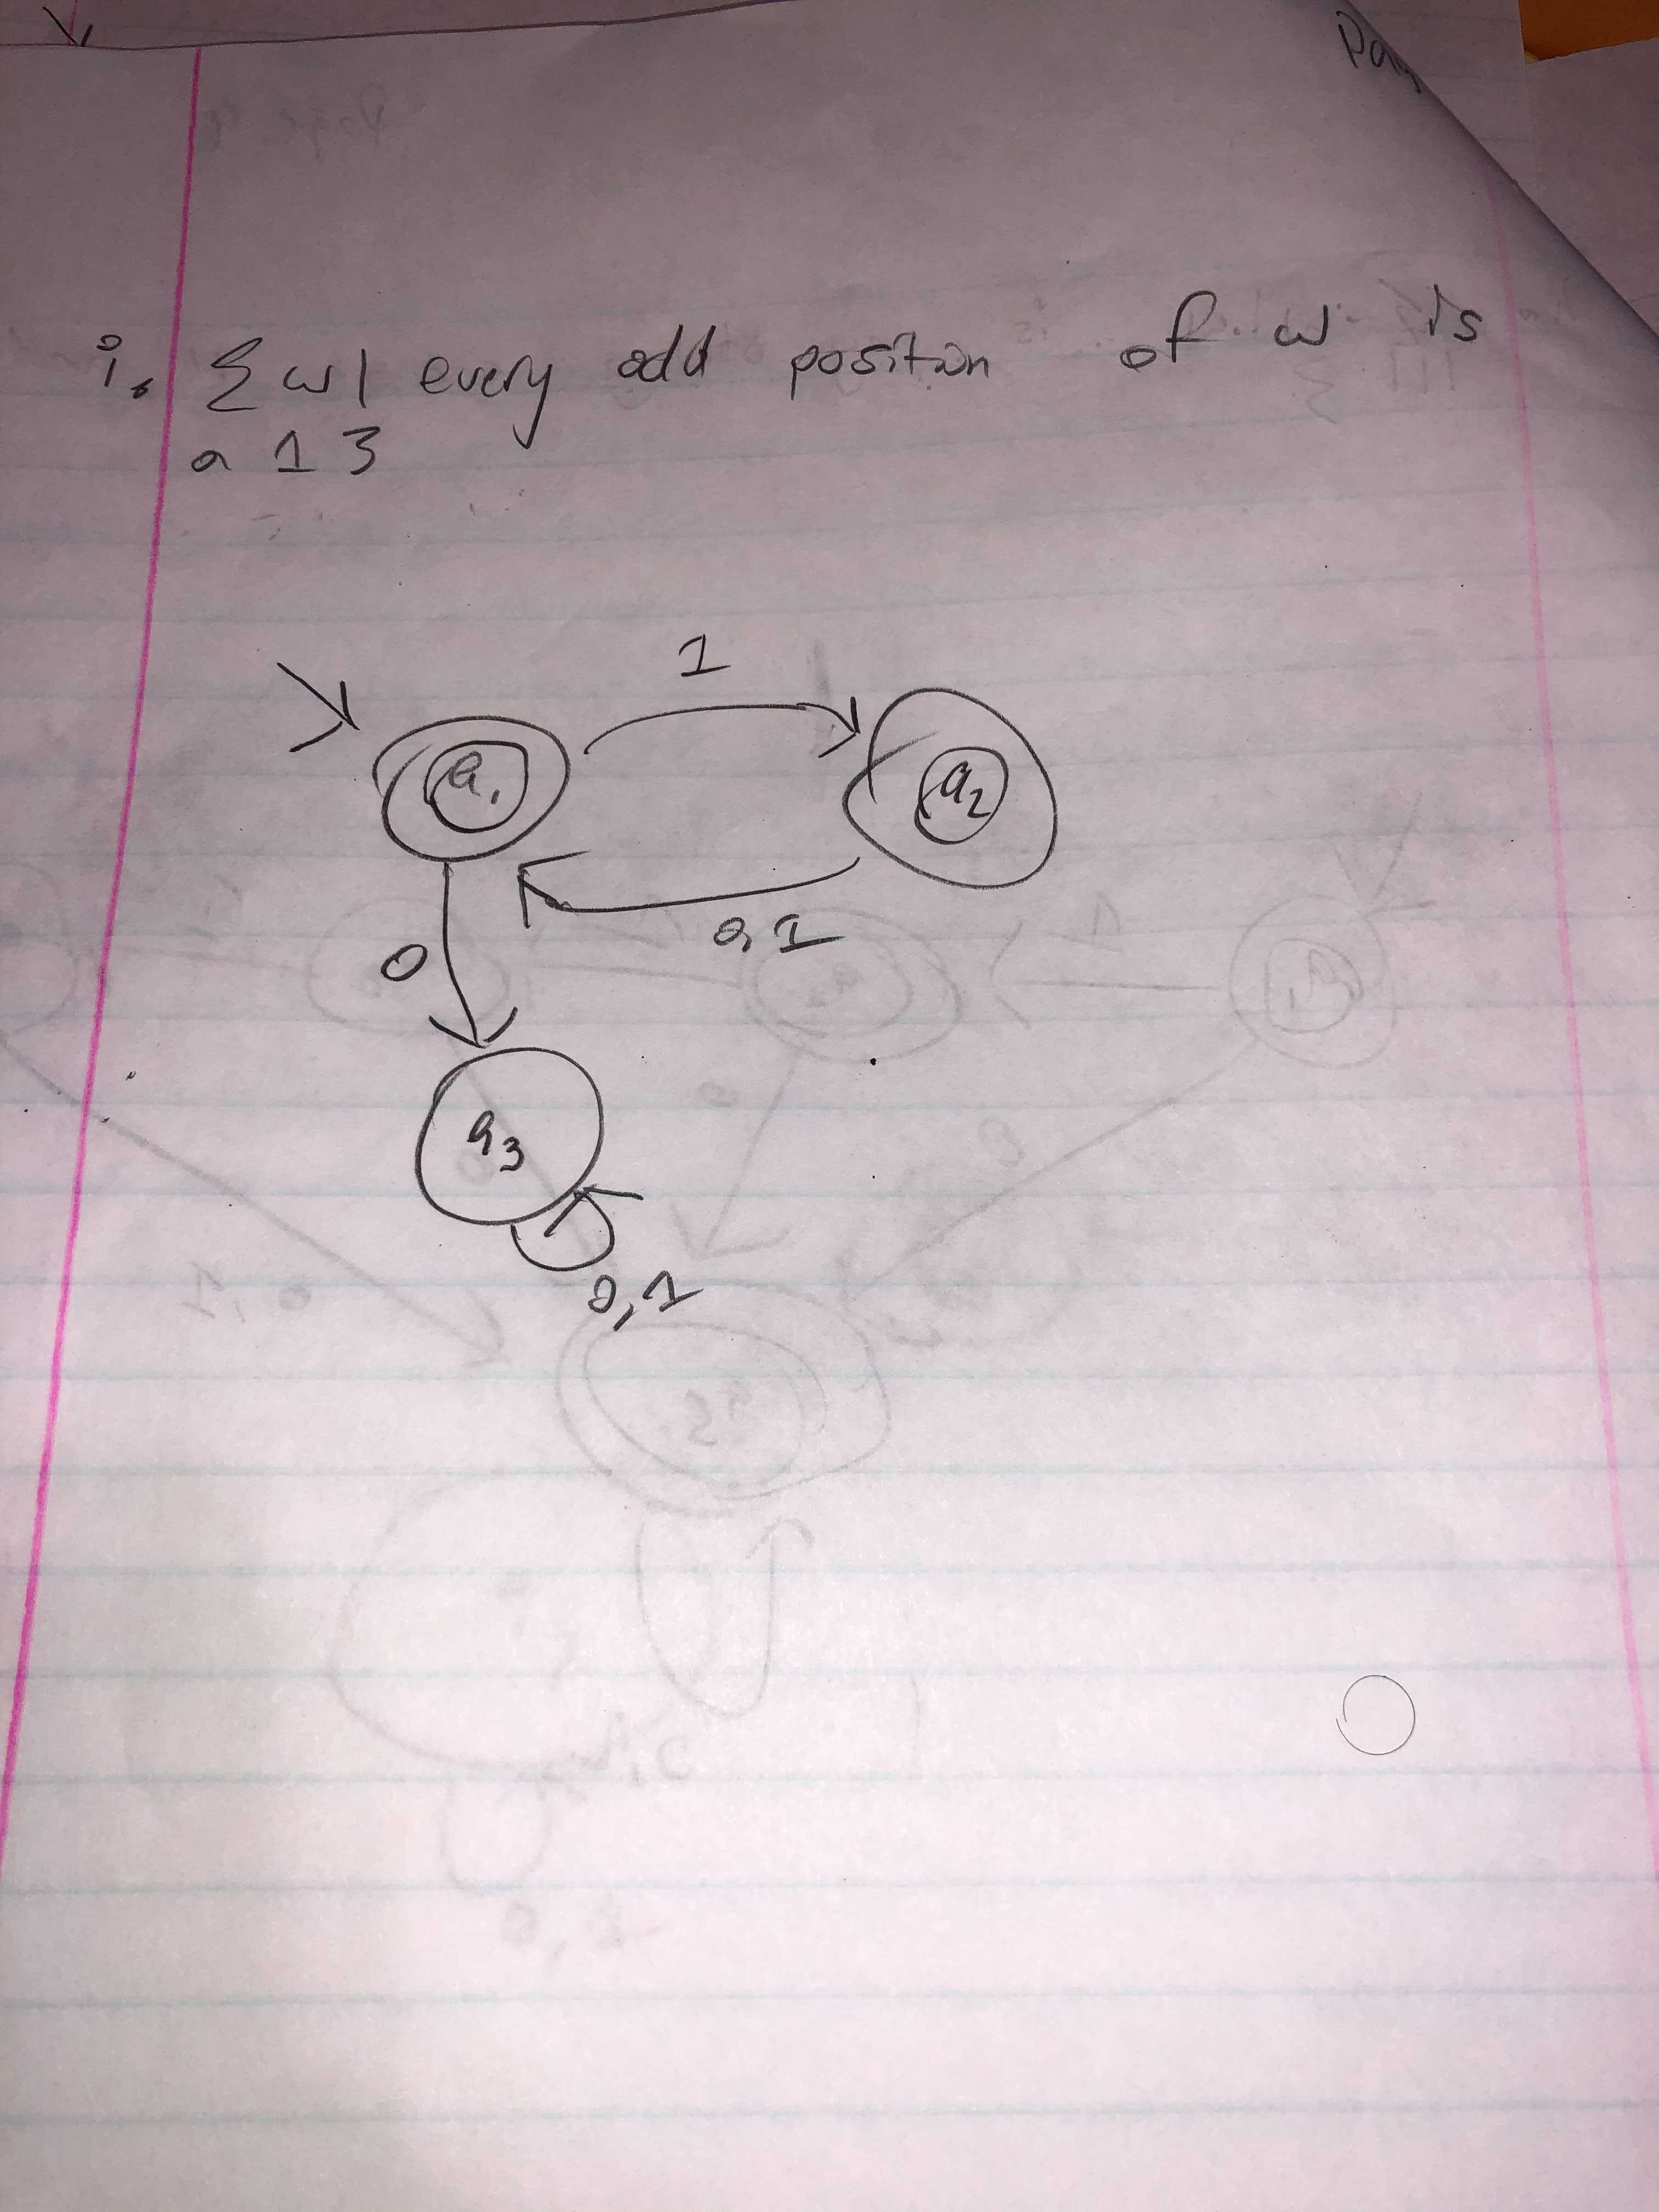
\includegraphics[width=15cm,height=15cm,keepaspectratio]{pics/page10}

j.

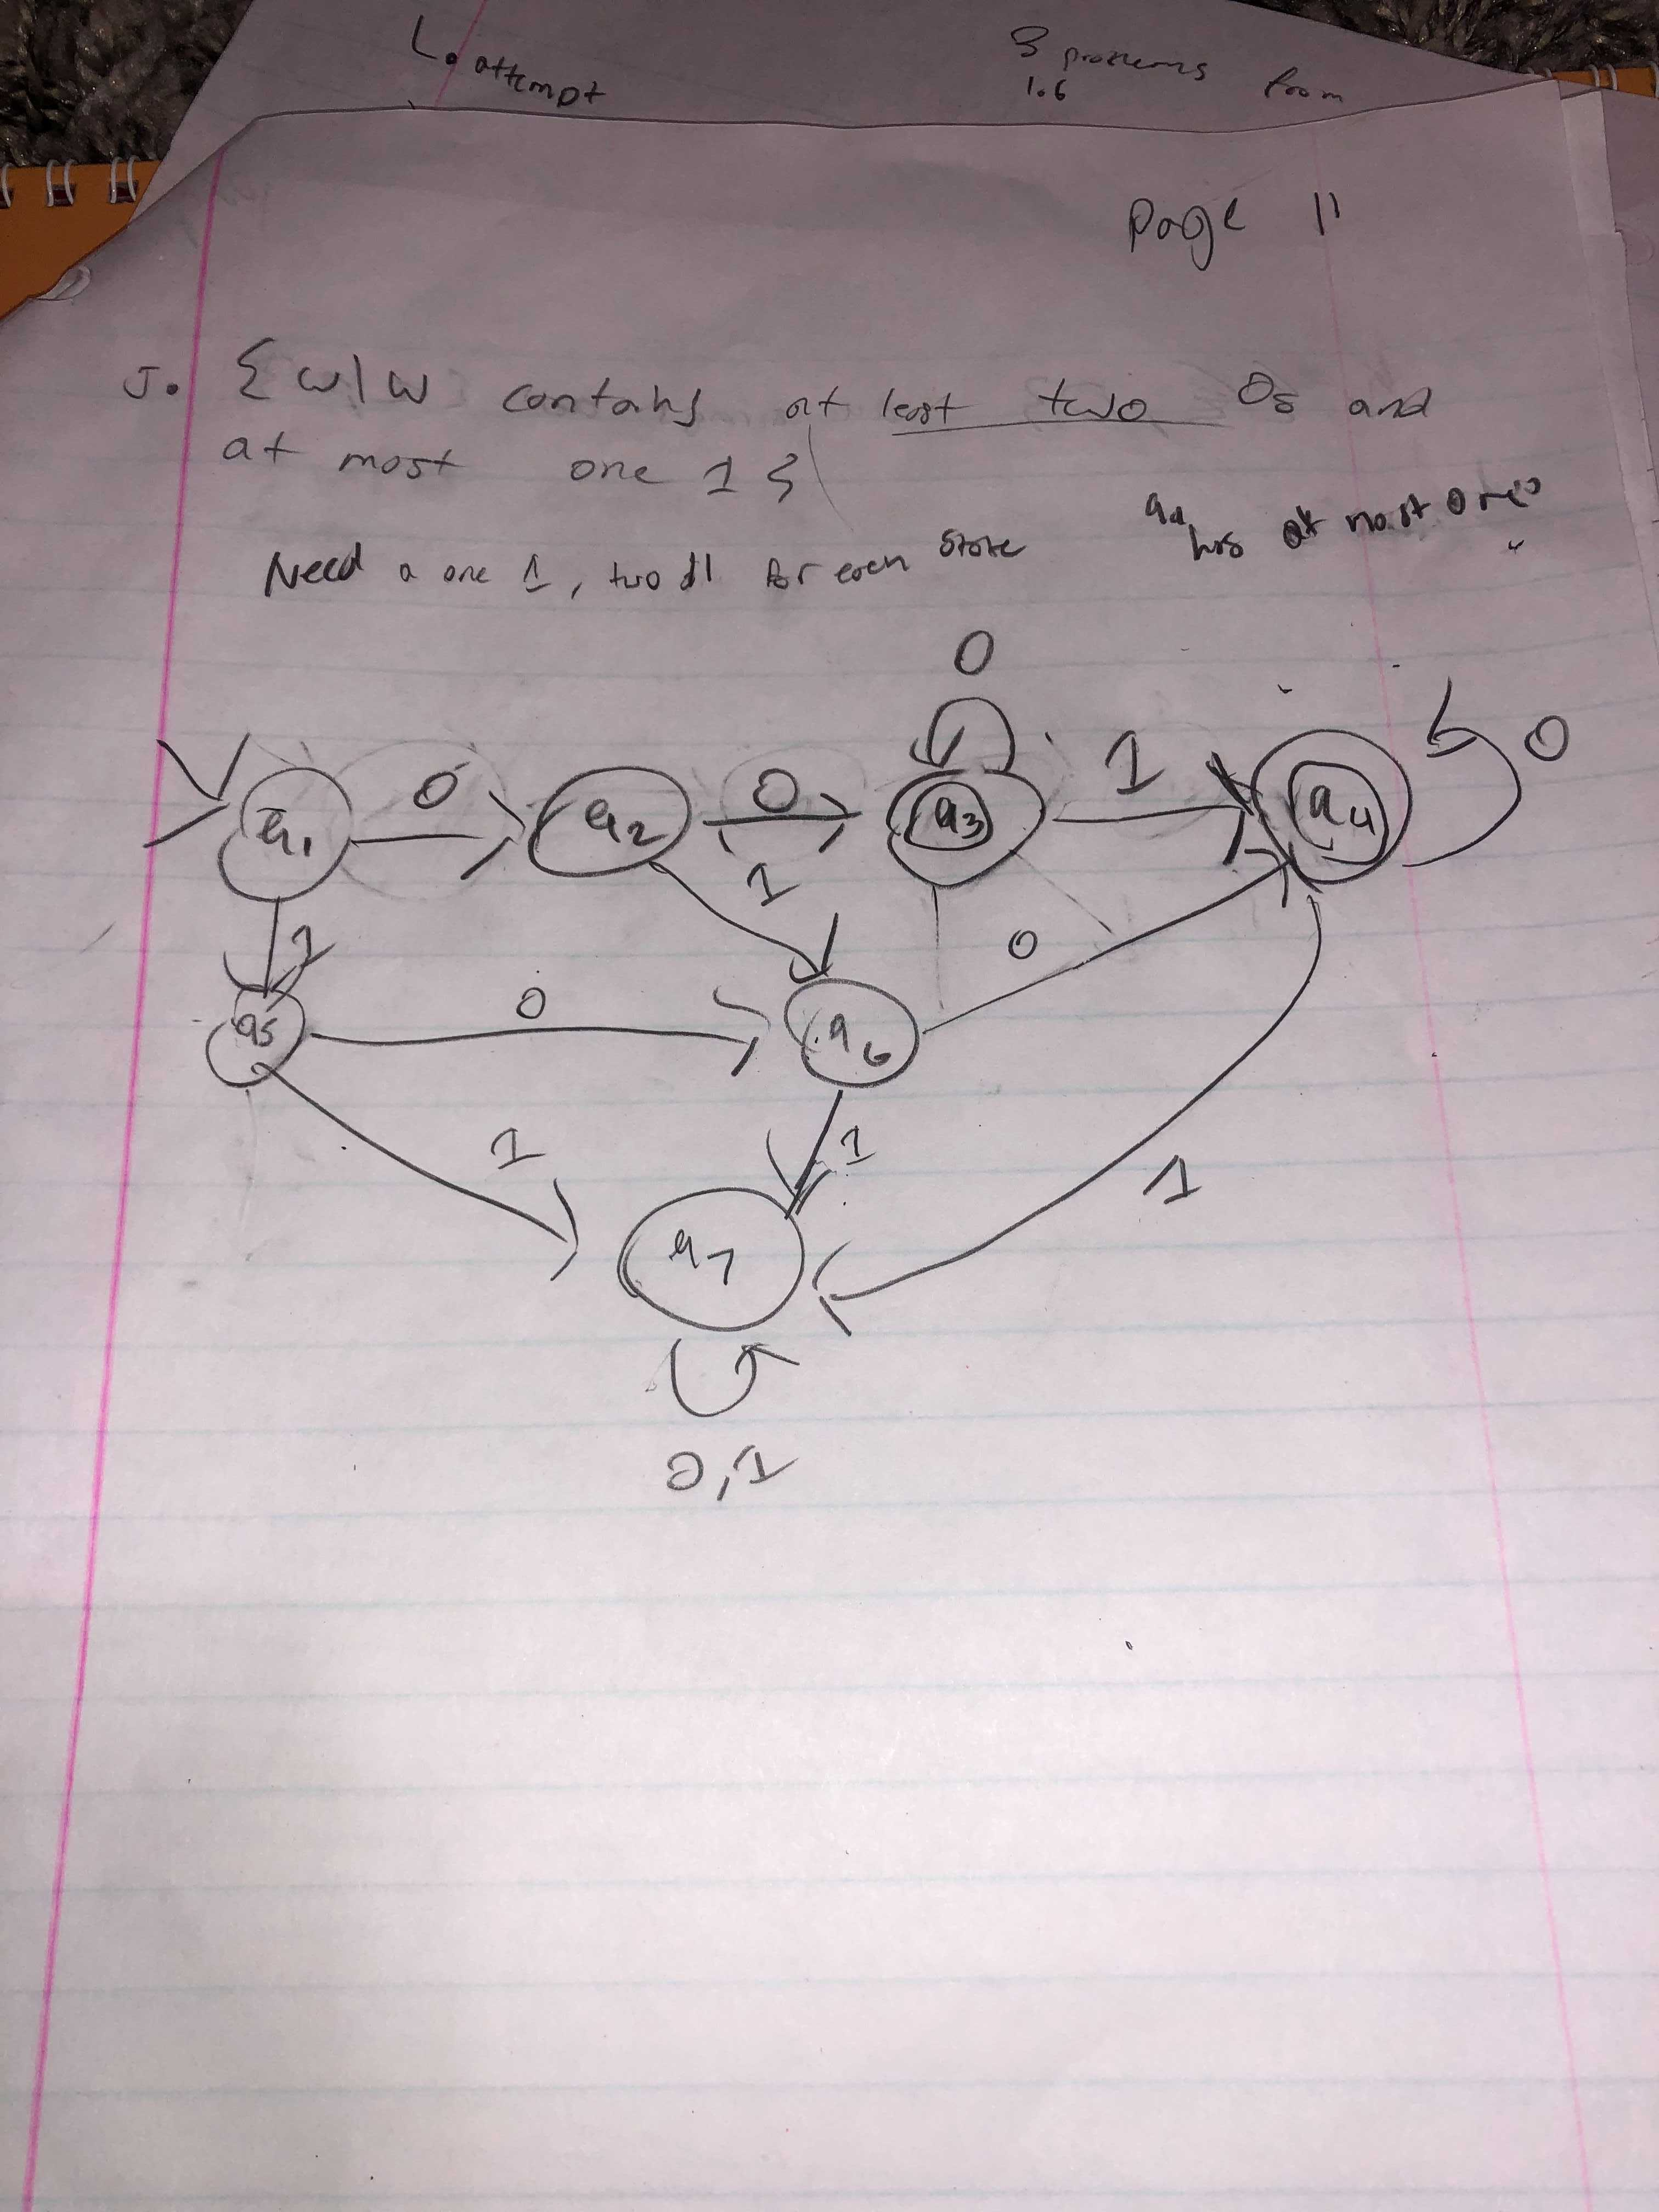
\includegraphics[width=15cm,height=15cm,keepaspectratio]{pics/pag11}

k.

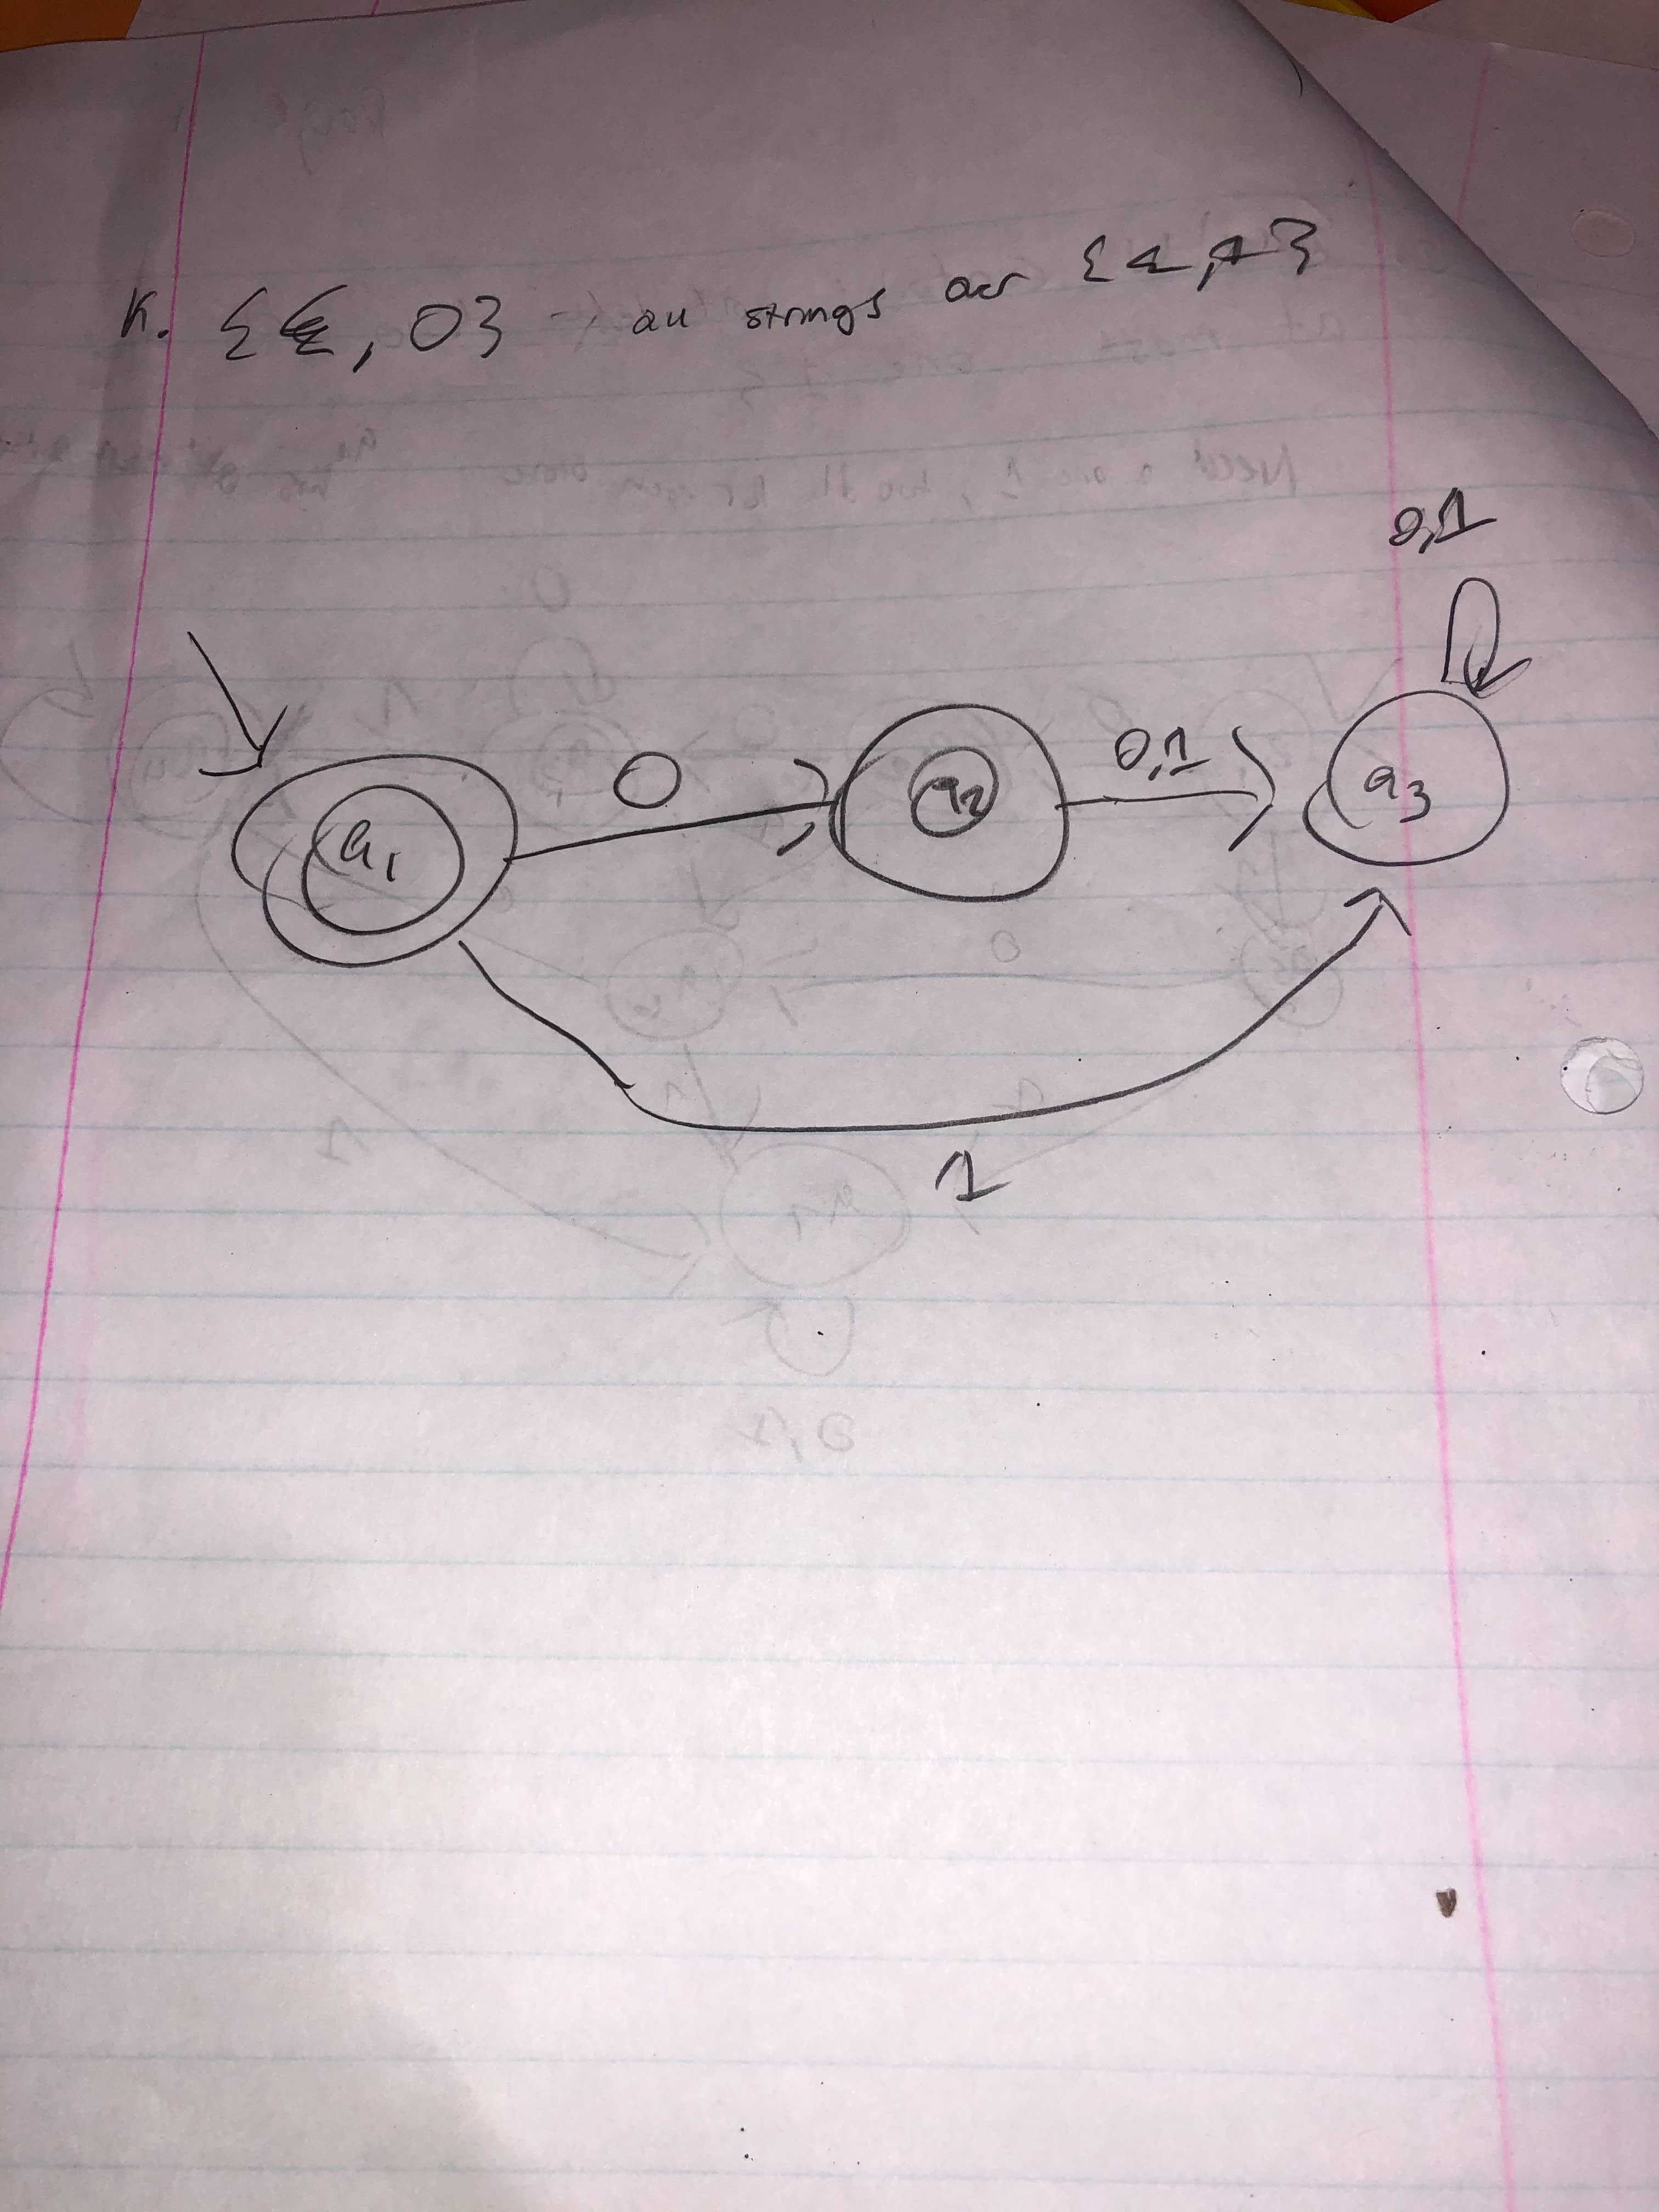
\includegraphics[width=15cm,height=15cm,keepaspectratio]{pics/page12}

l.

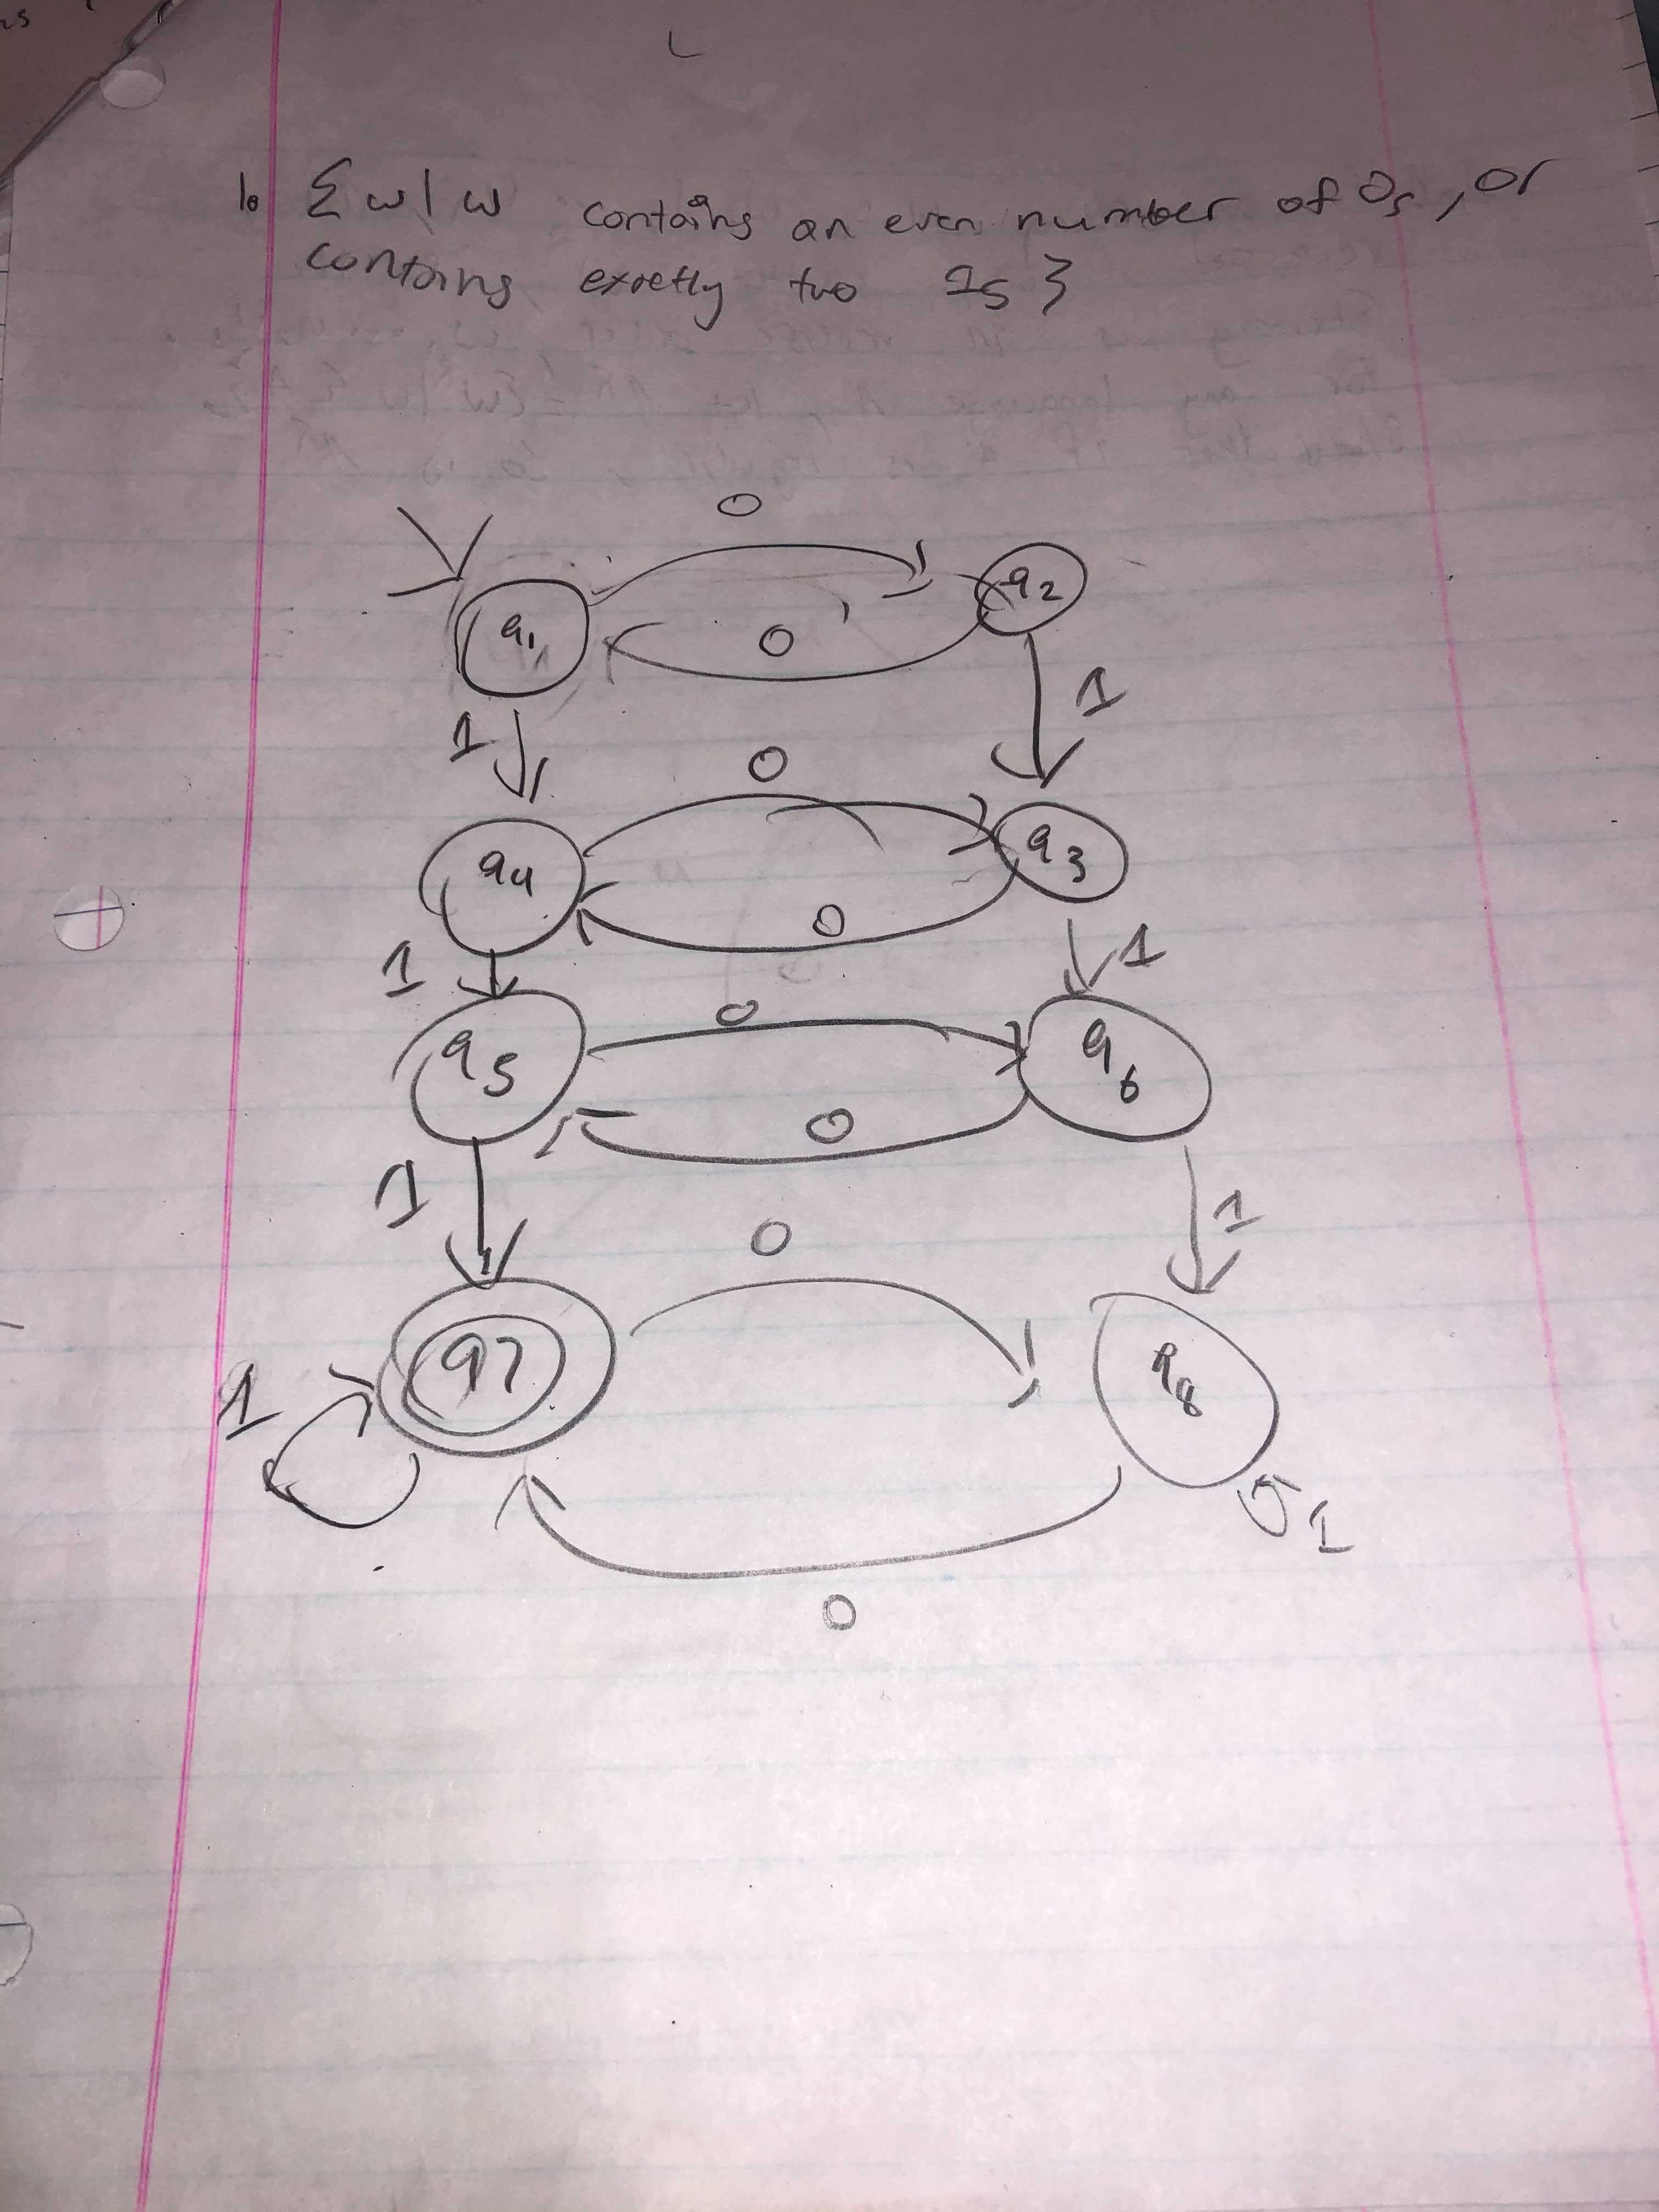
\includegraphics[width=15cm,height=15cm,keepaspectratio]{pics/page13}

1.31

First define $G$:

\includegraphics[width=15cm,height=15cm,keepaspectratio]{\string"/home/miguel/Downloads/Image from iOS\string".jpg}

In the picture, I defined the DFA using the bracket notation (please
see arrows to signify w1, w2, wn). The three dots signify that there
could be multiple arrows to represent different final states since
this DFA would be encapsulating any language and there is no set limit
of final states or arrows going into the states. Next, in order to
show the proof, I built an NFA for $G'$. I needed to: 

1. convert the start state as the only final state 

2. reverse the arrows of my DFA $G$

3. and make a new start date, named $q_{0}'$ that goes through $e$
input to get to the states to get the reverse string ($e$ because
we don't know the order so we consider all possibilities)

\includegraphics[width=15cm,height=15cm,keepaspectratio]{\string"/home/miguel/Downloads/Image from iOS (1)\string".jpg}

Here, you notice that $q0'$ = start state 

For any $w$ in all possiblities ($w$ in $\sum*$), there is a path
following $w$ from $q$$_{0}$$'$ to a final state $q$$_{0}$ $iff$
there is a path following $w^{R}$ from $q$$_{0}'$ to $q_{0}$in
$G'$. 

This means that $w$ in $A$ $iff$ $w^{R}$in $A^{R}$
\end{document}
